\documentclass[mat1]{fmfdelo}

\avtor{Aljaž Ostrež}

\naslov{Matrične potence}
\title{Powers of Matrices}

% mentorica, somentor
\mentorica{izr.~prof.~dr.~Marjeta Kramar Fijavž}
\somentor{doc.~dr.~Pavle Boškoski (Institut Jožef Stefan)}

\letnica{2021} % leto diplome

%  V povzetku na kratko opišite vsebinske rezultate dela. Sem ne sodi razlaga organizacije dela --
%  v katerem poglavju/razdelku je kaj, pač pa le opis vsebine.
\povzetek{V delu diplomskega seminarja obravnavamo matrične potence in zaporedja matričnih potenc. Sprva navedemo motivacijska zgleda in naredimo pregled pojmov iz linearne algebre, potrebnih za razumevanje besedila. Nato pogledamo matrične polinome in funkcije ter navedemo nekaj osnovnih pojmov iz spektralne teorije. V osrednjem delu si ogledamo koordinatna zaporedja, asimptotsko obnašanje matričnih zaporedij in Ces\`arovo konvergenco. Na koncu znanje, pridobljeno tekom diplomskega dela, uporabimo za analizo markovskih verig.}

%  Prevod slovenskega povzetka v angleščino.
\abstract{In the thesis we discuss matrix powers and sequences of matrix powers. We first give motivating examples and make an overview of the concepts from linear algebra needed to understand the text. We look at matrix polynomials and functions and list some basic concepts from spectral theory. In the central part, we look at coordinate sequences, asymptotic behavior of matrix sequences, and Ces\`aro summability. Finally, the knowledge gained during the thesis is used to analyze Markov chains.}

% navedite vsaj eno klasifikacijsko oznako --
% dostopne so na www.ams.org/mathscinet/msc/msc2020.html
\klasifikacija{15A16, 15A18, 60J10}
\kljucnebesede{matrika, matrične potence, markovska veriga, lastna vrednost, spektralni projektor, matrično zaporedje, Ces\`arova konvergenca} % navedite nekaj ključnih pojmov, ki nastopajo v delu
\keywords{matrix, powers of matrices, Markov chain, eigenvalue, spectal projection, matrix sequence, Ces\`aro summability} % angleški prevod ključnih besed

\zapisiMetaPodatke  % poskrbi za metapodatke in veljaven PDF/A-1b standard

% aktivirajte pakete, ki jih potrebujete
% \usepackage{tikz}
\usepackage{kbordermatrix}
\usepackage{graphicx}
\usepackage{mathtools}
\usepackage{commath}
\usepackage{dsfont}

% lokacija slik
\graphicspath{{./slike/}}

% za številske množice uporabite naslednje simbole
\newcommand{\R}{\mathbb R}
\newcommand{\N}{\mathbb N}
\newcommand{\Z}{\mathbb Z}
\newcommand{\C}{\mathbb C}
\newcommand{\Q}{\mathbb Q}

% matematične operatorje deklarirajte kot take, da jih bo Latex pravilno stavil
% \DeclareMathOperator{\conv}{conv}
\DeclareMathOperator{\Ima}{im}

% vstavite svoje definicije ...
%  \newcommand{}{}


\begin{document}

\section{Uvod}
Matrike so matematični objekti, ki so zelo uporabni v različnih vejah matematike in ostalih znanostih. V teoriji grafov matrika sosednosti enolično določa graf, ki je lahko utežen ali pa neutežen. V linearni algebri jih uporabljamo na primer za zapis linearnih preslikav med vektorskimi prostori in za proučevanje koeficientov sistemov linearnih enačb. V nadaljevanju bodo vse matrike kompleksne. To pomeni, da so koordinate matrike $A = [a_{ij}]_{1 \leq i,j \leq n}$ kompleksna števila, tj.\ $a_{ij} \in \C$ za $i,j = 1, \ldots, n$.

V nekaterih primerih pa nam poleg matrik pridejo prav tudi matrične funkcije. Eden od primerov matričnih funkcij je funkcija
\[f: \C^{n\times n} \rightarrow \C^{n\times n}\] s predpisom
\[f(A) = A^k\]
za $k\in\N$, kar je ravno $k$-ta potenca matrike $A\in\C^{n\times n}$. S pomočjo te funkcije lahko sestavimo zaporedje oblike $\left(A^k\right)_{k \in \N}$, ki je zelo uporabno v slučajnih procesih (stran \pageref{definicijaMarkov}). Želeli bomo opisati asimptotsko obnašanje matričnih zaporedij s splošnim členom $A_k = A^k$, kjer je $A \in \C^{n \times n}$. To obnašanje se lahko razbere že iz spektra matrike, včasih pa celo le iz spektralnega radija. Večino predstavljenih rezultatov povzemamo iz knjige \cite[2.~poglavje, 3.~poglavje, dod.~A]{kramar}.

Z naslednjimi zgledi bomo še dodatno motivirali uporabo matričnih potenc.
\subsection{Potence in Jordanova forma}
Najprej si poglejmo uporabo matričnih potenc na primeru Fibonaccijevega zaporedja.
\begin{zgled} [Fibonaccijevo zaporedje]
    Poznamo rekurzivno formulo za Fibonaccijevo zaporedje:
    \begin{align*}
        &f_0 = 0, f_1 = 1 \\
        &f_{n+1} = f_n + f_{n-1}, n \geq 1.
    \end{align*}
    Z uvedbo zaporedja $g_n = f_{n-1}$ dobimo sistem:
    \begin{align*}
        f_{n+1} &= f_n + g_n \\
        g_{n+1} &= f_n
    \end{align*}
    ob začetnih pogojih $f_1 = 1$ in $g_1 = 0$. Ta sistem lahko zapišemo v matrični obliki:
    \begin{equation*}
        \begin{bmatrix}
            f_{n+1} \\
            g_{n+1}
        \end{bmatrix}
        =
        \begin{bmatrix}
            1 & 1 \\
            1 & 0
        \end{bmatrix}
        \begin{bmatrix}
            f_n \\
            g_n
        \end{bmatrix}
    \end{equation*}
    za vsak $n \in \N$. Rekurzivno uporabljamo zgornji predpis, da dobimo
    \begin{equation*}
        \begin{bmatrix}
            f_{n+1} \\
            g_{n+1}
        \end{bmatrix}
        =
        \begin{bmatrix}
            1 & 1 \\
            1 & 0
        \end{bmatrix}
        \begin{bmatrix}
            f_n \\
            g_n
        \end{bmatrix}
        =
        \begin{bmatrix}
            1 & 1 \\
            1 & 0
        \end{bmatrix}
        ^2
        \begin{bmatrix}
            f_{n-1} \\
            g_{n-1}
        \end{bmatrix}
        = \cdots =
        \begin{bmatrix}
            1 & 1 \\
            1 & 0
        \end{bmatrix}
        ^n
        \begin{bmatrix}
            f_1 \\
            g_1
        \end{bmatrix}
    \end{equation*}
    oziroma
    \begin{equation*}
        \begin{bmatrix}
            f_{n+1} \\
            g_{n+1}
        \end{bmatrix}
        =
        \begin{bmatrix}
            f_{n+1} \\
            f_n
        \end{bmatrix}
        =
        \begin{bmatrix}
            1 & 1 \\
            1 & 0
        \end{bmatrix}
        ^n
        \begin{bmatrix}
            1 \\
            0
        \end{bmatrix}.
    \end{equation*}
    Z uporabo matričnih potenc torej lahko dobimo eksplicitno formulo za splošni člen v Fibonaccijevemu zaporedju
    \begin{equation*}
        f_n = a_{21},
    \end{equation*}
    kjer je $a_{21}$ prvi element v drugi vrstici matrike:
    \begin{equation*}
        A^n =
        \begin{bmatrix}
            1 & 1 \\
            1 & 0
        \end{bmatrix}
        ^n.
    \end{equation*}

    Tekom študija smo že spoznali en način za računanje matričnih potenc -- potence matrik lahko računamo s prevedbo na Jordanovo formo.

    Naj bo $A \in \C^{m\times m}$ matrika. Potem velja:
    \begin{equation*}
        A^n = PJ^nP^{-1},
    \end{equation*}
    kjer je $J$ Jordanova forma matrike $A$, $P$ pa pripadajoča prehodna matrika. Vemo, da je
    \begin{equation*}
        J^n = 
        \begin{bmatrix}
            J_1^n & & \\
            & \ddots & \\
            & & J_k^n
        \end{bmatrix},
    \end{equation*}
    kjer so $J_i, i=1,\ldots,k$, Jordanovi bloki. Za Jordanove bloke velja
    \begin{equation*}
        J_i^n = 
        \begin{bmatrix}
            \lambda_i^n & {n \choose 1}\lambda_i^{n-1} & \cdots & {n \choose m_i} \lambda_i^{n-m_i} \\
            & \lambda_i^n & \cdots  & {n \choose m_i-1} \lambda_i^{n-(m_i-1)} \\
            & & \ddots  & \vdots \\
            & & & \lambda_i^n
        \end{bmatrix},
    \end{equation*}
    pri čemer je $\lambda_i$ lastna vrednost matrike $A$, $m_i \times m_i$ pa velikost Jordanovega bloka.
    V posebnem primeru, ko je $J$ diagonalna matrika, velja:
    \begin{equation*}
        J^n = 
        \begin{bmatrix}
            \lambda_1^n & & \\
            & \ddots & \\
            & & \lambda_m^n
        \end{bmatrix}.
    \end{equation*}

    Z izračunom lastnih vrednosti in lastnih vektorjev bi za matriko:
    \begin{equation*}
        A = 
        \begin{bmatrix}
            1 & 1 \\
            1 & 0
        \end{bmatrix}
    \end{equation*}
    dobili Jordanovo formo (oziroma v tem primeru kar diagonalizacijo) matrike $A$ in prehodno matriko:
    \begin{equation*}
        J = 
        \begin{bmatrix}
                \frac{1+\sqrt{5}}{2} & 0 \\
            0 &  \frac{1-\sqrt{5}}{2}
        \end{bmatrix}
        ,\quad \quad
        P = 
        \begin{bmatrix}
            \frac{1-\sqrt{5}}{2} &  \frac{1+\sqrt{5}}{2} \vspace{2pt} \\
            1 & 1
        \end{bmatrix}.
    \end{equation*}
    Naš sistem enačb lahko zapišemo kot:
    \begin{equation*}
        \begin{bmatrix}
            f_{n+1} \\
            f_n
        \end{bmatrix}
        =
        A^n
        \begin{bmatrix}
            1 \\
            0
        \end{bmatrix}
        = PJ^n P^{-1}
        \begin{bmatrix}
            1 \\
            0
        \end{bmatrix}.
    \end{equation*}
    Izračunamo, da je:
    \begin{equation*}
        f_n = \frac{\sqrt{5}}{5}\left[ \left(\frac{1+\sqrt{5}}{2}\right)^n - \left(\frac{1-\sqrt{5}}{2}\right)^n \right], \quad n \in \N_0.
    \end{equation*}
    S pomočjo matričnih potenc smo iz rekurzivnega predpisa dobili eksplicitno formulo zaporedja.
\end{zgled}

Zakaj potrebujemo nove metode za računanje matričnih potenc, če jih že znamo računati s pomočjo Jordanove forme? Izkaže se, da je izračun Jordanove forme numerično zahteven, poleg tega pa nam Jordanova forma omogoča potenciranje matrik le v končnih dimenzijah. Velikokrat nam tudi ni potrebno izračunati celotne matrike $A^n$, ampak želimo le poznati nekatere njene lastnosti. Namesto Jordanove forme bomo uporabili spektralni razcep, ki ni odvisen od izbire baze matrike $A$.

\subsection{Markovske verige}\label{podpoglavjeMarkovskeVerige}

Uporabo matričnih potenc bomo prikazali na primeru markovskih verig. Navedimo definicijo markovske verige.
\begin{definicija}\label{definicijaMarkov}
    Naj bo $S$ števna množica, ki jo poimenujemo \emph{množica stanj}. Njene elemente $s \in S$ imenujemo \emph{stanja}. \emph{Slučajni proces} (z diskretnim časom) je vsako zaporedje diskretnih slučajnih spremenljivk $X_0, X_1, \ldots, X_n, \ldots$, katerih zaloga vrednosti leži v $S$. To zaporedje imenujemo \emph{markovska veriga}, če ima markovsko lastnost:
    \begin{equation*}
        P\left(X_n = s_n | X_0 = s_0, X_1 = s_1, \ldots, X_{n-1} = s_{n-1}\right) = P\left(X_n = s_n | X_{n-1} = s_{n-1}\right),
    \end{equation*}
    tj.\ verjetnost stanja na $n$-tem koraku je odvisna le od stanja na $(n-1)$-tem koraku. Vpeljemo še pojma \emph{prehodne verjetnosti na $n$-tem koraku}
    \begin{equation*}
        p_{ij} = P\left(X_n = s_j | X_{n-1} = s_i\right)
    \end{equation*}
    in \emph{prehodne matrike} $P = [p_{ij}]_{1 \leq i,j \leq n}$.
\end{definicija}
Poglejmo si zgled markovske verige, ki bo hkrati tudi motiviral računanje limite zaporedja $A_n = A^n$, če ta obstaja. 
\begin{zgled}
    Izberimo si vozlišče v poljubnem neusmerjenem grafu. Izberemo si naključnega soseda izbranega vozlišča in se premaknemo v njega. Postopek ponavljamo. Kolikšen je delež obiskov določenega vozlišča v grafu po dolgem času? Ker soseda izbiramo naključno, začetnemu grafu priredimo utežen usmerjen graf, kjer so uteži verjetnosti, da se premaknemo v povezanega soseda. Tu privzamemo, da so izbire sosedov enako verjetne, za vozlišče stopnje $k$ so vse verjetnosti enake $\frac{1}{k}$.
    \begin{figure}[!htb]
        \centering
        \begin{minipage}{0.5\textwidth}
            \centering
            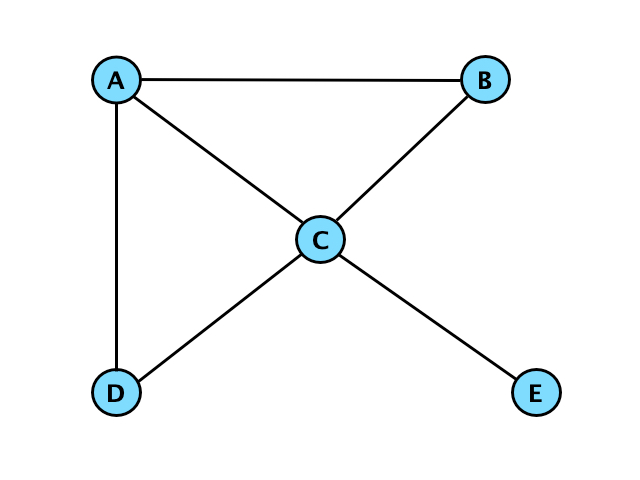
\includegraphics[width=\textwidth]{grafUndir.jpg}
            \caption{Začetni neusmerjen graf.}
        \end{minipage}
        \hspace{-30pt}
        \begin{minipage}{0.5\textwidth}
            % \vspace{30pt}
            \centering
            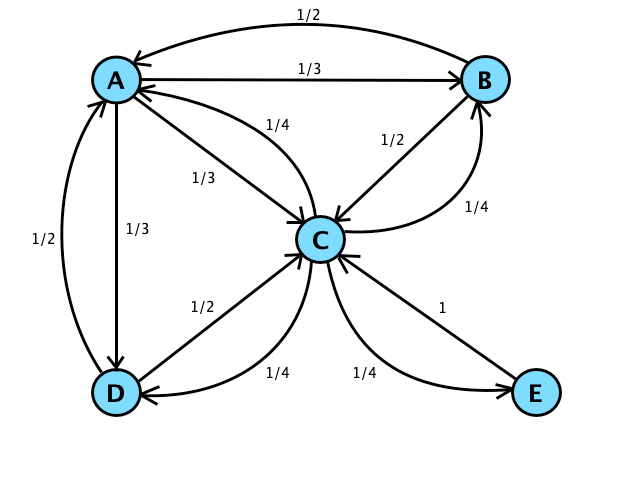
\includegraphics[width=\textwidth]{grafDir.jpg}
            \caption{Prirejen utežen usmerjen graf.}
        \end{minipage}
    \end{figure}

    \noindent Naša množica stanj je $S = \{A, B, C, D, E\}$, prehodna matrika pa bo kar matrika sosednosti prirejenega uteženega usmerjenega grafa
    \begin{equation*}
        P =
        \kbordermatrix{
                & A & B & C & D & E \\
            A & 0 & 1/3 & 1/3 & 1/3 & 0 \\
            B & 1/2 & 0 & 1/2 & 0 & 0 \\
            C & 1/4 & 1/4 & 0 & 1/4 & 1/4 \\
            D & 1/2 & 0 & 1/2 & 0 & 0 \\
            E & 0 & 0 & 1 & 0 & 0
        }.
    \end{equation*}
    Ker je izbira naslednjega vozlišča v zaporedju odvisna le od trenutnega vozlišča, ima naše zaporedje markovsko lastnost, torej bo naša pot v grafu markovska veriga. Kaj nam pa pove prehodna matrika?
    \begin{itemize}
        \item Vrstice matrike $P$ nam povejo, kolikšna je verjetnost, da bomo prišli v določeno vozlišče v naslednjem koraku, če smo trenutno v vozlišču, ki ga predstavlja vrstica.
        \item Vrstice matrike $P^2$ nam povejo, kolikšna je verjetnost, da bomo prišli v določeno vozlišče čez $2$ koraka.
        \item ...
        \item Vrstice matrike $P^n$ nam povejo, kolikšna je verjetnost, da bomo prišli v določeno vozlišče čez $n$ korakov.
    \end{itemize}
    Za naš primer se izkaže celo, da obstaja limita:
    \begin{equation*}
        \lim_{n \rightarrow \infty} P^n =
        \begin{bmatrix}
            0{,}25 & 0{,}17 & 0{,}33 & 0{,}17 & 0{,}08 \\
            0{,}25 & 0{,}17 & 0{,}33 & 0{,}17 & 0{,}08 \\
            0{,}25 & 0{,}17 & 0{,}33 & 0{,}17 & 0{,}08 \\
            0{,}25 & 0{,}17 & 0{,}33 & 0{,}17 & 0{,}08 \\
            0{,}25 & 0{,}17 & 0{,}33 & 0{,}17 & 0{,}08 
        \end{bmatrix}.
    \end{equation*}
    Ta limita nam pove delež obiskov za vsako vozlišče (če bi zelo dolgo potovali). Limita je tudi neodvisna od izbire začetnega vozlišča, če je le graf krepko povezan \cite[Theorem 5.1]{markov}.
\end{zgled}

\subsection{Ponovitev iz linearne algebre}\label{linearnaAlgebra}
Naj bo $A \in \C^{n \times n}$ matrika dimenzije $n \times n$. Definirajmo \emph{množico polinomov matrike} $A$ s predpisom
\begin{equation*}
    \mathcal{P}_A := \left\{ \sum_{i=0}^m \alpha_i A^i\ |\  \alpha_i \in \C, m \in \N_0 \right\} \subset \C^{n \times n}.
\end{equation*}
Če je $p(x) = \sum_{i=0}^m \alpha_i x^i$ polinom, bomo pisali
\begin{equation*}
    p(A) := \sum_{i=0}^m \alpha_i A^i.
\end{equation*}
Definirajmo preslikavo
\begin{align}
\begin{split}
    \Phi_A : \C [x] &\longrightarrow \mathcal{P}_A \\
    p &\longmapsto p(A),
\end{split}
\end{align}
kjer je $\C [x]$ množica polinomov s koeficienti iz $\C$. Jedro preslikave $\Phi_A$ je
\begin{equation*}
    \ker \left(\Phi_A\right) = \Big\{ p \in \C [x] \ | \  p(A) = 0 \Big\},
\end{equation*}
torej, $\ker\left(\Phi_A\right)$ je množica vseh polinomov, za katere je $p(A) = 0$.

\begin{definicija}
    \emph{Minimalni polinom} $m_A \in \C[x]$ je neničeln monični polinom najmanjše stopnje iz $\ker\left(\Phi_A\right)$, tj.\ monični polinom $p$ najnižje stopnje, za katerega je $p(A) = 0$.
\end{definicija}
\begin{opomba}
    \emph{Monični polinom} je polinom z vodilnim koeficientom enakim $1$.
\end{opomba}
Spomnimo se, da je minimalni polinom $m_A$ enolično določen z matriko $A$. Potrebovali bomo še pojem \emph{lastne vrednosti} in \emph{lastnega vektorja} matrike $A$, osvežimo pa še definicijo \emph{karakterističnega polinoma} matrike $A$. Poleg tega navedimo še definicijo \emph{lastnega podprostora}.
\begin{definicija}
    Naj bo $A \in \C^{n\times n}$.
    \begin{enumerate}
        \item Število $\lambda \in \C$ imenujemo \emph{lastna vrednost} matrike $A$, če obstaja tak vektor $x \in \C^n$, $x \neq 0$, da velja
        \begin{equation*}
            Ax = \lambda x.
        \end{equation*}
        Vektorji $x$, za katere velja zgornja enačba, so pripadajoči \emph{lastni vektorji}.
        \item \emph{Lastni podprostor} matrike $A$, ki pripada lastni vrednosti $\lambda$, je definiran kot $\ker \left(A - \lambda I\right)$.
        \item Polinom
        \begin{equation*}
            \Delta_A(\lambda) = \det \left(A - \lambda I\right) \in \mathcal{P}_A
        \end{equation*}
        v spremenljivki $\lambda$ imenujemo \emph{karakteristični polinom} matrike $A$.
        \item \emph{Algebraična večkratnost} lastne vrednosti $\lambda$ je večkratnost $\lambda$ kot ničle polinoma $\Delta_A\left(\lambda\right)$, \emph{geometrična večkratnost} lastne vrednosti $\lambda$ pa večkratnost $\lambda$ kot ničle minimalnega polinoma $m_A\left(\lambda\right)$.
    \end{enumerate}
\end{definicija}
Matrika $A - \lambda I$ je \emph{nilpotentna} reda $\nu$, kjer je $\nu$ geometrična večkratnost lastne vrednosti $\lambda$. To pomeni, da velja $\left(A - \lambda I\right)^k = 0$ za $k \geq \nu$.

Brez dokaza se spomnimo naslednje trditve, s pomočjo katere med drugim tudi na roke iščemo lastne vrednosti matrike $A$.
\begin{trditev}
    Naj bo $A \in \C^{n \times n}$, $m_A$ pripadajoči minimalni polinom, $\Delta_A$ pripadajoči karakteristični polinom in $\lambda \in \C$. Naslednje trditve so ekvivalentne:
    \begin{enumerate}
        \item $\lambda$ je lastna vrednost matrike $A$,
        \item matrika $A- \lambda I$ ni obrnljiva,
        \item $\lambda$ je ničla polinoma $m_A$,
        \item $\lambda$ je ničla polinoma $\Delta_A$.
    \end{enumerate}
\end{trditev}

Iz zgornje trditve sledi, da lahko minimalni polinom $m_A$ matrike $A$ zapišemo kot
\begin{equation*}
    m_A(z) = \left(z-\lambda_1\right)^{\nu_1}\left(z-\lambda_2\right)^{\nu_2}\cdots \left(z-\lambda_m\right)^{\nu_m},
\end{equation*}
kjer so $\lambda_1, \ldots, \lambda_m$ lastne vrednosti matrike $A$, $\nu_1, \ldots, \nu_m$ pa pripadajoče geometrične večkratnosti.

V nadaljevanju bomo omenjali tudi \emph{matrične} in \emph{operatorske norme}, zato se spomnimo lastnosti norme.
\begin{definicija}
    \emph{Matrična norma} na $\C^{n \times n}$ je takšna preslikava $\norm{\cdot}: \C^{n \times n} \rightarrow \R$, da za vsaki matriki $A, B \in \C^{n \times n}$ in vsak skalar $\alpha \in \C$ velja:
    \begin{enumerate}
        \item $\norm{A} \geq 0$ in $\norm{A} = 0$ natanko tedaj, ko je $A = 0$ (pozitivnost),
        \item $\norm{\alpha A} = |\alpha|\norm{A}$ (homogenost),
        \item $\norm{A + B} \leq \norm{A} + \norm{B}$ (trikotniška neenakost), 
        \item $\norm{A B} \leq \norm{A} \norm{B}$ (submultiplikativnost).
    \end{enumerate}
    Matrične norme, ki so porojene iz vektorskih norm s predpisom
    \begin{equation*}
        \norm{A} = \max_{x \neq 0} \frac{\norm{A x}}{\norm{x}}\quad \text{za}\ x\in \C^n,
    \end{equation*}
    imenujemo \emph{operatorske norme}.
\end{definicija}
\begin{zgled}
    Matrične norme, ki so porojene iz vektorskih $p$-norm, imenujemo \emph{$p$-norme}. To so operatorske norme in so definirane kot
    \begin{equation*}
        \norm{A}_p = \max_{x \neq 0} \frac{\norm{A x}_p}{\norm{x}_p},
    \end{equation*}
    kjer je $A \in \C^{n\times n}$. Dva predstavnika $p$-norm, ki imata še posebej poenostavljen predpis, sta:
    \begin{itemize}
        \item \emph{1-norma}, ki je definirana kot
        \begin{equation*}
            \norm{A}_1 = \max_{1 \leq j \leq n} \sum_{i=1}^n |a_{ij}|,
        \end{equation*}
        tj.\ največja od vsot absolutnih vrednosti elementov v istem stolpcu,
        \item \emph{$\infty$-norma}, ki je definirana kot
        \begin{equation*}
            \norm{A}_\infty = \max_{1 \leq i \leq n} \sum_{j=1}^n |a_{ij}|,
        \end{equation*}
        tj.\ največja od vsot absolutnih vrednosti elementov v isti vrstici. \qedhere
    \end{itemize}
\end{zgled}
Operatorska norma je torej podrazred matričnih norm in ima nekaj zanimivih lastnosti.
\begin{trditev}\label{trditevOperatorska}
    Naj bo $A \in \C^{n \times n}$, $x \in \C^{n \times n}$ in $\norm{\cdot}$ operatorska norma na $\C^{n \times n}$. Potem velja
    \begin{equation*}
        \norm{A x} \leq \norm{A} \cdot \norm{x}.
    \end{equation*}
\end{trditev}
\begin{dokaz}
    Za $x = 0$ trditev očitno velja. Za $x \neq 0$ pa velja
    \begin{equation*}
        \frac{\norm{A x}}{\norm{x}} \leq \max_{x \neq 0} \frac{\norm{A x}}{\norm{x}} = \norm{A},
    \end{equation*}
    torej je $\norm{A x} \leq \norm{A} \cdot \norm{x}$.
\end{dokaz}
\begin{posledica}\label{posledicaOperatorskaNorma}
    Naj bo $A \in \C^{n \times n}$ in $\norm{\cdot}$ neka operatorska norma na $\C^{n \times n}$. Potem velja neenakost
    \begin{equation*}
        \norm{A} \geq \max\{|\lambda|\ |\ \lambda\  \text{je lastna vrednost matrike}\  A\}.
    \end{equation*}
\end{posledica}
\begin{dokaz}
    Po definiciji lastne vrednosti velja $A x = \lambda x$ za neki lastni vektor $x \in \C^{n \times n}$, $x \neq 0 $. Zato velja tudi
    \begin{equation*}
        \norm{A x} = \norm{\lambda x} = |\lambda|\cdot \norm{x}.
    \end{equation*}    
    Ker je $\norm{\cdot}$ operatorska norma, po trditvi \ref{trditevOperatorska} velja
    \begin{equation*}
        \norm{A x} \leq \norm{A} \cdot \norm{x}.
    \end{equation*}
    Sledi, da je
    \begin{equation*}
        |\lambda|\cdot \norm{x} \leq \norm{A} \cdot \norm{x},
    \end{equation*}
    torej je $|\lambda| \leq \norm{A}$. To velja za vsako lastno vrednost $\lambda$. Posledica sledi.
\end{dokaz}


\begin{definicija}
    Matrika $P \in \C^{n \times n}$ je \emph{projektor}, če velja $P^2 = P$.
\end{definicija}
\begin{zgled}
    Poglejmo si primer pravokotnega projektorja v prostoru $\R^3$. Za pravokotni projektor velja, da je $\ker P \bot \Ima P$. Projicirajmo vektor $v = (1,1,0)$ pravokotno na ravnino $\Sigma$, ki je podana z enačbo $x + y + z = 0$. Naj bo $n = (1,1,1)$ normalni vektor te ravnine, ki ni normiran. Vemo, da s formulo
    \begin{equation}\label{eqProjekcijaVektor}
        \operatorname{proj}_{n}(v) = \frac{n \cdot v}{n\cdot n}\cdot n
    \end{equation}
    projiciramo vektor $v$ na vektor $n$. S tem lahko izračunamo tudi projekcijo vektorja $v$ na ravnino $\Sigma$.
    \begin{figure}[H]
        \vspace{-10pt}
        \centering
        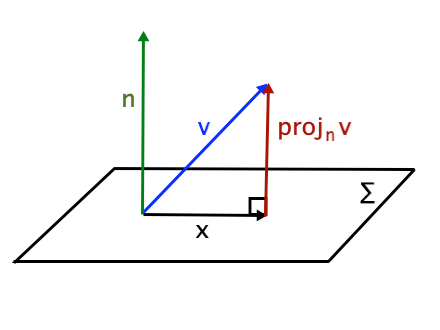
\includegraphics[width=0.5\textwidth]{projekcija.jpg}
        \vspace{-25pt}
        \caption{Projekcija vektorja $v$ na ravnino $\Sigma$.}
    \end{figure}
    Če vstavimo $v$ in $n$ v formulo \eqref{eqProjekcijaVektor}, dobimo
    \begin{equation*}
        \operatorname{proj}_{n}(v) = \frac{2}{3}\cdot (1,1,1).
    \end{equation*}
    Ker velja $x = v - \operatorname{proj}_{n}(v)$, je torej
    \begin{equation*}
        x = \operatorname{proj}_\Sigma (v) = \frac{1}{3}\cdot (1,1,-2).
    \end{equation*}
    Bolj zanimiv kot le izračun $\operatorname{proj}_\Sigma (v)$ pa je izračun projektorja, ki vektor $v$ projicira na vektor $n$. Če pišemo skalarni produkt kot množenje matrik, tj.\ $a\cdot b = a^T \cdot b$, iz asociativnosti matričnega množenja sledi
    \begin{equation*}
        \operatorname{proj}_{n}(v) = \frac{n^T  v}{n^T n}\cdot n = \frac{\left(n^T  v\right)n}{n^T n} = \frac{n\left(n^T  v\right)}{n^T n} = \frac{n  n^T}{n^T n}\cdot v.
    \end{equation*}
    S $P$ označimo matriko $\frac{n  n^T}{n^T n}$. V našem primeru izračunamo, da je
    \begin{equation*}
        P = \frac{1}{3}\cdot
        \begin{bmatrix}
            1 & 1 & 1 \\
            1 & 1 & 1 \\
            1 & 1 & 1
        \end{bmatrix},
    \end{equation*}
    velja pa tudi $P^2 = P$, kar pomeni, da je $P$ res projektor. Enačba $\operatorname{proj}_n (v) = P v$ pa sledi direktno iz izpeljave.
\end{zgled}
\begin{definicija}
    Naj bosta $X$ in $Y$ vektorska prostora nad $\C$, za katera velja \\ $X \cap Y = \emptyset$. Tedaj vsoti
    \begin{equation*}
        X + Y = \{x+y \ |\ x\in X, y\in Y\}
    \end{equation*}
    pravimo \emph{direktna vsota} in jo označimo z $X \oplus Y$.
\end{definicija}
\begin{trditev}
    Matrika $P \in \C^{n \times n}$ je projektor natanko tedaj, ko je
    \begin{equation*}
        \C^n = \ker P \oplus \Ima P\quad  \text{in}\quad P|_{\Ima P} = I.
    \end{equation*}
\end{trditev}
\begin{dokaz}
    $(\Leftarrow)$$\quad P|_{\Ima P} = I$ implicira $P\left(P x\right) = P x$ za vsak $x \in \C^n$, tj.\ $P^2 = P$, kar je ravno definicija projektorja.

    $(\Rightarrow)$Naj bo $x \in \C^n$ in $y \in \Ima P$, tako da velja $y = P x$. Definirajmo $z := x-y$. Potem je $x = z + y$ in
    \begin{equation*}
        P z = P x - P y = P x - P^2 x = P x - P x = 0,
    \end{equation*}
    torej je $z\in \ker P$. Lahko sklepamo tudi, da iz $y \in \Ima P$ sledi $P y = P^2 x = P x = y$.

    Dokažimo še, da je razcep na direktno vsoto enoličen. Naj bosta $y' \in \Ima P$ in $z' \in \ker P$ takšna, da je $x = y' + z'$. Iz računa
    \begin{equation*}
        y = P x = P y' + P z' = y'
    \end{equation*}
    sledi, da je $y = y'$ in $z = z'$.
\end{dokaz}

\section{Spektralni razcep in matrične funkcije}
\subsection{Matrični polinomi}
V podpoglavju \ref{linearnaAlgebra} smo že definirali množico matričnih polinomov $\mathcal{P}_A$ in minimalni polinom $m_A$ matrike $A \in \C^{n \times n}$, pa tudi preslikavo $\Phi_A$ iz množice polinomov $\C [x]$ v $\mathcal{P}_A$.
\begin{trditev}\label{trditevMinimalniPolinom}
    Naj bo $m_A$ minimalni polinom matrike $A$. Potem je
    \begin{equation*}
        p \in \ker \left(\Phi_A\right) \Leftrightarrow p = m_A \cdot q\ \  \text{za}\ \ q \in \C [x],
    \end{equation*}
    tj.\ $p(A) = 0$ natanko tedaj, ko je $p(A)$ večkratnik minimalnega polinoma $m_A$.
\end{trditev}
\begin{dokaz}
    Najprej dokažimo implikacijo ($\Leftarrow$). Če je $p = m_A\cdot q$ za neki $q \in \C [x]$, potem je
    \begin{equation*}
        p(A) = m_A(A) \cdot q(A) = 0 \cdot q(A) = 0,
    \end{equation*}
    torej je $p \in \ker\left(\Phi_A\right)$.
    
    Dokažimo še ($\Rightarrow$). Naj bo $p \in \C [x]$, za katerega velja $p(A) = 0$. Če delimo $p$ z $m_A$, dobimo:
    \begin{equation*}
        p = m_A \cdot q + r
    \end{equation*}
    za $q, r \in \C [x]$, kjer je $\text{st}(r) < \text{st}\left(m_A\right)$. Ker je $m_A(A) = 0$, velja
    \begin{equation*}
        0 = p(A) = m_A(A) \cdot q(A) + r(A) = r(A),
    \end{equation*}
    torej je $r \in \ker\left(\Phi_A\right)$. Ker ima $m_A$ najmanjšo stopnjo v $\ker\left(\Phi_A\right)$, sklepamo, da je $r = 0$.
\end{dokaz}

Za polinome $p, q, r \in \C [x]$ bomo uporabljali zapis
\begin{equation*}
    p \equiv q \mod r\  \Longleftrightarrow\  p - q = s\cdot r\ \  \text{za neki}\  s\in \C [x].
\end{equation*}
Poglejmo si posledico trditve \ref{trditevMinimalniPolinom}
\begin{posledica} \label{posledicaProjekcija}
    Za $p, q \in \C [x]$ velja
    \begin{equation*}
        p(A) = q(A)\  \Longleftrightarrow\ p \equiv q \mod m_A.
    \end{equation*}
    V posebnem primeru velja, da je $p(A)$ projektor natanko tedaj, ko je
    \begin{equation*}
        p^2 \equiv p \mod m_A.
    \end{equation*}
\end{posledica}
Opazimo torej, da je lahko $p(A) = q(A)$ tudi, če polinoma $p, q \in \C [x]$ nista enaka. Naslednja trditev pa nam pove, da lahko enakost po po modusu $m_A$ preverimo le s pomočjo lastnih vrednosti matrike $A$ in njihovih večkratnosti.
\begin{trditev} \label{trditevPosploseniMinimalni}
    Naj bosta $p, q \in \C [x]$ in naj bodo $\lambda_1,\ldots,\lambda_m$ ničle minimalnega polinoma $m_A$ z večkratnostmi $\nu_1,\ldots,\nu_m$. Potem velja
    \begin{equation*}
        p \equiv q \mod m_A \ \Longleftrightarrow\  p^{\left(\nu\right)}\left(\lambda_i\right) = q^{\left(\nu\right)}\left(\lambda_i\right)\ \text{za vsak}\ i = 1, \ldots, m\ \text{in}\ \nu = 0, \ldots, \nu_i-1.
    \end{equation*}
\end{trditev}
\begin{dokaz}
    Trditev sledi iz dejstva, da za neki $n\in \N$ in neničeln $s \in \C [x]$ ter fiksen $\lambda_i \in \C$ velja
    \begin{equation*}
        \left(p-q\right)(x) = \left(x-\lambda_i\right)^n s(x) \ \Longleftrightarrow\  \left(p-q\right)^{(\nu)}(\lambda_i)=0 \ \text{za}\  i=0, 1, \ldots, n-1,
    \end{equation*}
    kar smo že dokazali pri študiju algebre \cite[poglavje 7.5]{bresar}.
\end{dokaz}

\subsection{Gladke matrične funkcije}

Naj bo $A \in \C^{n\times n}$ matrika z minimalnim polinomom $m_A$ ter $\lambda_1, \ldots, \lambda_m$ ničle $m_A$ z večkratnostmi $\nu_1, \ldots, \nu_m$. Množico funkcij, ki so definirane in neskončnokrat odvedljive na neki okolici $\{\lambda_1, \ldots, \lambda_m\}$, označimo kot
\begin{equation*}
    C_A^\infty := \{ f: D(f) \rightarrow \C\ |\ \exists U \subset D(f)\ \text{odprta}, \{\lambda_1, \ldots, \lambda_m\} \subset U, f|_U \in C^\infty \},
\end{equation*}
kjer je $D(f) \subset \C$ definicijsko območje funkcije $f$.

Pri uporabi funkcije $f \in \C_A^\infty$ na matriki $A$ si bomo pomagali z interpolacijskimi polinomi. \emph{Interpolacijski polinom} je polinom stopnje največ $n$, ki se v $n+1$ točkah $(x_0, f(x_0)), (x_1, f(x_1)), \ldots, (x_n, f(x_n))$ ujema s funkcijo $f$. Če zahtevamo, da se za $i=0, \ldots, n$ v točkah $(x_i, f(x_i)$ ujemajo tudi vsi odvodi do $k_i$-tega, pa je stopnja interpolacijskega polinoma navzgor omejena z $\sum_{i=0}^n (k_i + 1) - 1$.
\begin{definicija} \label{definicijaGladkaFunkcija}
    Za $f \in \C_A^\infty$ definiramo matriko $f(A)$ s pomočjo interpolacijskega polinoma:
    \begin{equation*}
        f(A) := \Phi_A(p_f) = p_f(A),
    \end{equation*}
    kjer je $p_f$ polinomska interpolacija funkcije $f$, ki zadošča pogoju
    \begin{equation*}
        f^{(\nu)}(\lambda_i) = p_f^{(\nu)}(\lambda_i)
    \end{equation*}
    za vsak $i = 1, \ldots, m$ in $\nu = 0, \ldots, \nu_i-1$.
\end{definicija}
S to definicijo lahko matrične polinome razširimo na množico gladkih matričnih funkcij:
\begin{align}
    \begin{split}
        \widetilde{\Phi}_A :\ &C_A^\infty \longrightarrow \mathcal{P}_A \\
        &\widetilde{\Phi}_A(f) = \Phi_A(p_f) = p_f(A)
    \end{split}
\end{align}
Iz definicije \ref{definicijaGladkaFunkcija} in trditev \ref{trditevMinimalniPolinom}, \ref{trditevPosploseniMinimalni} sledijo naslednje lastnosti.
\begin{trditev} \label{trditevPhiAlgebra}
    Naj bodo oznake kot zgoraj. Potem veljajo naslednje trditve:
    \begin{enumerate}
        \item Definicija $\widetilde{\Phi}_A(f)$ ni odvisna od izbire metode za polinomsko interpolacijo $p_f$.
        \item Preslikava $\widetilde{\Phi}_A$ je razširitev funkcije $\Phi_A$.
        \item $\widetilde{\Phi}$ je homomorfizem algeber, kar pomeni, da velja:
        \begin{align*}
            \widetilde{\Phi}_A(\lambda f + \mu g) &= \lambda \widetilde{\Phi}_A(f) + \mu \widetilde{\Phi}_A(g), \\
            \widetilde{\Phi}_A(f \cdot g) &= \widetilde{\Phi}_A(f) \cdot \widetilde{\Phi}_A(g)
        \end{align*}
        za $\lambda, \mu \in \C$ in $f, g \in C_A^\infty$.
    \end{enumerate}
\end{trditev}
Za odprto množico $U \subset \C$ definirajmo \emph{karakteristično funkcijo} $\chi_U$ s predpisom
\begin{equation*}
    \chi_U(\lambda) =
    \begin{cases}
        1, \lambda \in U, \\
        0, \lambda \notin U
    \end{cases}.
\end{equation*}
Funkcija $\chi_U$ je idempotentna, kar pomeni, da velja $\chi_U \cdot \chi_U = \chi_U$. Po posledici \ref{posledicaProjekcija} sklepamo, da je $\chi_U(A) \in \mathcal{P}_A$ projektor, ki komutira z A. Vzemimo posebno množico takšnih projektorjev.
\begin{definicija}\label{Uimnozice}
Naj bodo $U_1, \ldots, U_m \subset \C$ odprte množice, ki zadostujejo pogojema:
\begin{enumerate}
    \item $\lambda_i \in U_i$ za $i = 1,\ldots,m$ in
    \item $U_i \cap U_j = \emptyset$ za $i \neq j$.
\end{enumerate}
S $\chi_i$ označimo karakteristično funkcijo množice $U_i$. Matrike
\begin{equation} \label{definicijaProjekcije}
    P_i := \chi_i(A) \in \mathcal{P}_A\ \text{za}\ i = 1,\ldots, m,
\end{equation}
so vse projektorji, ki jih imenujemo \emph{spektralni projektorji}, njihovo zalogo vrednosti pa označimo kot 
\begin{equation} \label{zalogeProjekcij}
    X_i := \Ima P_i = P_i \C^n.
\end{equation}
\end{definicija}
\begin{opomba}
    \leavevmode
    \begin{enumerate}
        \item Omenimo, da je $P_i$ neodvisna od izbire $U_i$, poleg tega pa velja še $P_i \neq 0$ za vsak $i$.
        \item Poznamo formulo za izračun spektralnih projektorjev diagonalizabilnih matrik \cite[7.~poglavje, str.~529, enačba 7.3.11]{meyer}. Če je $A$ diagonalizabilna matrika z lastnimi vrednostmi $\lambda_1, \ldots, \lambda_m$, potem spektralni projektor za lastno vrednost $\lambda_i$ izračunamo kot:
        \begin{equation}\label{spektralniProjektorjiDiag}
            P_i = \prod_{\substack{\ j=1 \\ j \neq i}}^m \frac{A-\lambda_j I}{\lambda_i-\lambda_j}, \quad i=1, \ldots, m.
        \end{equation}
    \end{enumerate}
\end{opomba}

Za naslednji izrek moramo razumeti pojem invariantnosti.
\begin{definicija}
    Podprostor $Y$ prostora $X$ je \emph{invarianten za $A$} oz.\ \emph{$A$-invarianten}, kadar velja $A y \in Y$ za vsak $y \in Y$, kar lahko zapišemo kot $A Y \subseteq Y$.
\end{definicija}
Projektorji $P_i$ komutirajo z $A$, zato so podprostori $X_i$ invariantni za $A$, in velja naslednje. 
\begin{izrek}\label{trditevSpektralniRazcep}
    Naj bo $A \in \C^{n \times n}$ matrika z lastnimi vrednostmi $\lambda_1, \ldots, \lambda_m$ z geometrijskimi večkratnostmi $\nu_1, \ldots, \nu_m$. Če vzamemo $P_i$ in $X_i$ kot v \eqref{definicijaProjekcije} in \eqref{zalogeProjekcij}, potem je
    \begin{equation}\label{eqSpektralniRazcep}
        \C^n = X_1 \oplus \cdots \oplus X_m
    \end{equation}
    direktni razcep na $A$-invariantne podprostore z lastnostjo, da je matrika $A - \lambda_i I$ na $X_i$ nilpotentna reda $\nu_i$, $i = 1, \ldots, m$.
\end{izrek}
\begin{dokaz}
    Ker so množice $U_i$ iz definicije \ref{Uimnozice} disjunktne, velja $\chi_i\left(\sum_{i \neq j} \chi_j\right) = 0$, torej tudi $P_i\left(\sum_{i \neq j} P_j\right) = 0$. Iz tega sledi, da je
    \begin{equation*}
        X_i \cap \left(\bigoplus_{i \neq j} X_j\right) = \{0\}.
    \end{equation*}
    Ker je $\{\lambda_1, \ldots, \lambda_m\} \subset \bigcup_{i = 1}^m U_i =: U$, je
    \begin{equation*}
        \sum_{i = 1}^m P_i = \widetilde{\Phi}_A \left(\sum_{i=1}^m \chi_i \right) = \widetilde{\Phi}_A (\chi_U) = I,
    \end{equation*}
    torej je $X_1 \oplus \cdots \oplus X_m = X$.
    
    Spomnimo, da je matrika $A$ nilpotentna reda $k$, če velja $A^k = 0$ in $A^{k-1} \neq 0$. Za vsak fiksen $i$ je $g_i(\lambda) = (\lambda - \lambda_i)^{\nu_i} \chi_i(\lambda)$ funkcija v domeni preslikave $\widetilde{\Phi}_A$, ki se v točkah $\lambda_1, \ldots, \lambda_m$ ujema z ničelno funkcijo $\mathbb{O} \in C_A^{\infty}$, vključno z vsemi odvodi. Zaradi lastnosti $\widetilde{\Phi}_A$ iz trditve \ref{trditevPhiAlgebra} in definicije \ref{definicijaGladkaFunkcija} mora veljati
    \begin{equation*}
        (A - \lambda I)^{\nu_i} P_i = \left(\left(\lambda - \lambda_i \right)^{\nu_i} \chi_i \right) (A) = \mathbb{O}(A) = 0
    \end{equation*}
    za $i = 1, \ldots, m$ in $\lambda \in \C$. Definirajmo funkcijo
    \begin{equation*}
        f_i(\lambda) = (\lambda - \lambda_i)^{\nu_i - 1} \chi_i(\lambda),\ \lambda \in \C.
    \end{equation*}
    Ker je
    \begin{equation*}
        f_i^{(\nu_i-1)} (\lambda_i) \neq 0,
    \end{equation*}
    velja $f_i(A) = (A - \lambda_i I)^{\nu_i-1} P_i \neq 0$, torej je matrika $A - \lambda_i I$ nilpotentna reda $\nu_i$ na $X_i$.
\end{dokaz}
\begin{definicija}
    Razcepu $\C^n$ na invariante podprostore iz formule \eqref{eqSpektralniRazcep} rečemo \emph{spektralni razcep} prostora $\C^n$, ki pripada matriki $A$. 
\end{definicija}
Spektralni razcep nam pove, da je matrika $A$ podobna bločno diagonalni matriki,
\begin{equation*}
    A \sim
    \begin{bmatrix}
       A_1 & & \\
       & \ddots & \\
       & & A_m 
    \end{bmatrix},
\end{equation*}
kjer ima $A_i$ eno samo lastno vrednost, in sicer $\lambda_i$. Iz tega dejstva bi lahko slutili, da bi za podprostore $X_i$ vzeli kar korenske podprostore $\ker (A - \lambda_i I)^{\nu_i}$ za lastne vrednosti $\lambda_i$.
\begin{trditev}
    $X_i$ so korenski podprostori matrike $A$ za lastne vrednosti $\lambda_i$:
    \begin{equation*}
        X_i = \ker (A - \lambda_i I)^{\nu_i},
    \end{equation*}
    kjer je $\nu_i$ geometrijska večkratnost lastne vrednosti $\lambda_i$.
\end{trditev}
\begin{dokaz}
    Trditev \ref{trditevSpektralniRazcep} nam pove, da je $A - \lambda_i I$ nilpotentna reda $\nu_i$ na $X_i$, zato je
    \begin{equation} \label{strogaVsebovanost}
        X_i \subset \ker (A - \lambda_i I)^{\nu_i}.
    \end{equation}
    Recimo, da je vsebovanost stroga, tj.\ obstaja neničeln vektor $x \in \ker (A - \lambda_i I)^{\nu_i} \backslash X_i$. Za neki $j \neq i$ potem obstaja $y \neq 0,\ y := P_j x \in X_j \cap \ker (A - \lambda_i I)^{\nu_i}$. Vzemimo največje število $p \in \N$, za katerega velja
    \begin{equation*}
        z := (A - \lambda_i I)^p y \neq 0.
    \end{equation*}
    Ker je $X_j$ $A$-invarianten, je $z \in X_j$. Iz
    \begin{equation*}
        (A - \lambda_i I) z = (A - \lambda_i I)^{p+1} y = 0
    \end{equation*}
    sledi, da je $z$ lastni vektor za lastno vrednost $\lambda_i$, tj.\ $A z = \lambda_i z$, iz česar sledi, da
    \begin{equation*}
        (A - \lambda_j I)^{\nu_j} z = \left(A - \lambda_i I + \lambda_i I - \lambda_j I\right)^{\nu_j} z = (\lambda_i - \lambda_j)^{\nu_j} z \neq 0,
    \end{equation*}
    kar je v protislovju z lastnostjo, da je $A - \lambda_j I$ na $X_j$ nilpotentna reda $\nu_j$.
\end{dokaz}

S pomočjo spektralnega razcepa v izreku \ref{trditevSpektralniRazcep} lahko izračunamo $f(A)$ brez iskanja interpolacijskih polinomov.
\begin{izrek} \label{trditevFormula}
    Naj bo $A \in \C^{n \times n}$ z lastnimi vrednostmi $\lambda_1, \lambda_2, \ldots, \lambda_m$, ki imajo po vrsti večkratnosti $\nu_1, \nu_2, \ldots, \nu_m$. Definirajmo projektorje $P_i$ kot v \eqref{definicijaProjekcije}. Tedaj za vsako funkcijo $f \in C_A^\infty$ velja
    \begin{equation*}
        f(A) = \sum_{i=1}^m \sum_{\nu = 0}^{\nu_i - 1} \frac{f^{(\nu)}(\lambda_i)}{\nu !}(A - \lambda_i)^\nu P_i.
    \end{equation*}
\end{izrek}
\begin{dokaz}
    Funkcija
    \begin{equation*}
        g(\lambda) = \sum_{i=1}^m \sum_{\nu = 0}^{\nu_i - 1} \frac{f^{(\nu)}(\lambda_i)}{\nu !}(\lambda - \lambda_i)^\nu \chi_i(\lambda), \quad \lambda \in \C,
    \end{equation*}
    sovpada z $f$, vključno z vsemi pomembnimi odvodi, na vseh točkah $\lambda_1, \ldots, \lambda_m$.  Po trditvah \ref{trditevPosploseniMinimalni}, \ref{trditevPhiAlgebra} in definiciji \ref{definicijaGladkaFunkcija} sledi, da je $f(A) = g(A)$.
\end{dokaz}
\begin{posledica}
    Naj bodo predpostavke enake kot v izreku \ref{trditevFormula}. Za $k \in \N$ velja
    \begin{equation}\label{formulaMatricnePotence}
        A^k = \sum_{i=1}^m \sum_{\nu = 0}^{\min \{\nu_i - 1, k\}} {k \choose \nu} \lambda_i^{k-\nu}(A - \lambda_i)^\nu P_i.
    \end{equation}
\end{posledica}
\begin{dokaz}
    V izreku \ref{trditevFormula} za $k \in \N$ uporabimo funkcijo $f(\lambda) = \lambda^k$.
\end{dokaz}

\subsection{Spektralna teorija}
Tu zberimo še nekaj rezultatov o spektru matrik, ki jih bomo kasneje potrebovali.
\begin{definicija}
    Naj bo $A \in \C^{n \times n}$. Množico
    \begin{equation*}
        \sigma(A) := \{\lambda_1, \ldots, \lambda_m\}
    \end{equation*}
    imenujemo \emph{spekter} matrike A. \emph{Spektralni radij} definiramo kot
    \begin{equation*}
        r(A) := \max \{|\lambda|\ |\ \lambda \in \sigma(A)\},
    \end{equation*}
    tj.\ absolutna vrednost največje lastne vrednosti matrike $A$.
\end{definicija}

Naslednja trditev nam pove, kako se preslika spekter matrike za neko preslikavo iz $C_A^\infty$.
\begin{izrek} [Izrek o preslikavi spektra]\label{izrekOPreslikaviSpektra}
    Naj bo $A \in \C^{n \times n}$ in $f \in C_A^\infty$. Potem velja
    \begin{equation*}
        \sigma\left(f\left(A\right)\right) = f\left(\sigma\left(A\right)\right) := \{f(\lambda)\ |\ \lambda \in \sigma(A)\}.
    \end{equation*}
\end{izrek}
\begin{dokaz}
    Naj bo $\lambda$ poljubna lastna vrednost matrike $A$ in $\mu \notin f(\sigma(A))$. Definirajmo $u(\lambda) := \frac{1}{f(\lambda) - \mu} \in C_A^\infty$, torej je $u(\lambda) \cdot (f(\lambda) - \mu) = 1$ na okolici $\sigma(A)$. Če v to enačbo vstavimo matriko $A$, dobimo
    \begin{equation*}
        u(A) \cdot (f(A) - \mu I) = (f(A) - \mu I) \cdot u(A) = I,
    \end{equation*}
    torej je matrika $f(A) - \mu I$ obrnljiva, zato $\mu \notin \sigma(f(A))$.
    
    Obratno, naj bo $x_i$ lastni vektor matrike $A$, ki pripada lastni vrednosti $\lambda_i$ za $i = 1, \ldots, m$. Po izreku \ref{trditevSpektralniRazcep} za vse $i \neq j$ velja $P_j x_i = 0$ in $P_i x_i = x_i$. Po izreku \ref{trditevFormula} sledi
    \begin{equation*}
        f(A) x_i = f(\lambda_i) x_i,
    \end{equation*}
    torej je $f(\lambda_i) \in \sigma(f(A))$.
\end{dokaz}

\begin{lema}\label{lemaNorme}
    Naj bo $\norm{\cdot}$ norma na $\C^{n \times n}$. Za $A \in \C^{n \times n}$ in $\mu > r(A)$ obstajata konstanti $N > 0$ in $M > 1$, da za vse $k \in \N$ velja
    \begin{equation*}
        N \cdot r(A)^k \leq \norm{A^k} \leq M \cdot \mu^k.
    \end{equation*}
    Če je $\norm{\cdot}$ operatorska norma, lahko izberemo $N = 1$.
\end{lema}
Dokaz zgornje leme bo sledil v nadaljevanju (na strani \pageref{dokazLemaNorme}). Iz te leme sledi zanimiva formula, s pomočjo katere lahko spektralni radij matrike izračunamo s pomočjo matričnih potenc.
\begin{trditev} [Gelfandova formula] \label{gelfand}
    Za matriko $A \in \C^{n \times n}$ velja naslednje.
    \begin{enumerate}
        \item $r(A) = \lim_{k \rightarrow \infty} \norm{A^k}^{1/k}$ za vsako matrično normo $\norm{\cdot}$ na $\C^{n \times n}$.
        \item Če je $\norm{\cdot}$ operatorska norma na $\C^{n \times n}$, potem je $r(A) = \inf_{k > 0} \norm{A^k}^{1/k}$.
    \end{enumerate}
\end{trditev}

\begin{dokaz}
    Če vzamemo $k$-ti koren enačbe iz leme \ref{lemaNorme}, dobimo oceno:
    \begin{equation*}
        N^{1/k} r(A) \leq \norm{A^k}^{1/k} \leq M^{1/k} \mu
    \end{equation*}
    za vsak $\mu > r(A)$ in in za določeni konstanti $N, M$. Če je $\norm{\cdot}$ operatorska norma, za dopustno izbiro $N = 1$ dobimo
    \[r(A) = \inf_{k > 0} \norm{A^k}^{1/k}. \qedhere\]
\end{dokaz}


\section{Zaporedja matričnih potenc}
V tem poglavju bomo opazovali asimptotsko obnašanje matričnih zaporedij oblike $(A^k)_{k\in\N}$. Izkazalo se bo, da nekatere lastnosti lahko karakteriziramo s spektralnim radijem matrike $A$. Da pridemo do tega rezultata, moramo najprej povedati nekaj o koordinatnih zaporedjih.
\subsection{Koordinatna zaporedja}
\begin{lema}\label{lemaNeodvisnost}
    Naj bo $A \in \C^{n \times n}$ z lastnimi vrednostmi $\lambda_1, \ldots, \lambda_m$ z geometrijskimi večkratnostmi $\nu_1, \ldots, \nu_m$.
    \begin{enumerate}
        \item Za $i = 1, \ldots, m$ in $0\neq z \in X_i$ je množica
                 \begin{equation*}
                     \{(A-\lambda_i I)^{\nu} z\ |\ \nu = 0, \ldots, \nu_i - 1\} \backslash \{0\}
                 \end{equation*}
                linearno neodvisna v $X_i$.
        \item Množica
                 \begin{equation*}
                     B_A = \{(A-\lambda_i I)^{\nu} P_i\ |\ i = 1, \ldots, m;\ \nu = 0, \ldots, \nu_i - 1\}
                 \end{equation*}
                je linearno neodvisna v $\C^n$.
    \end{enumerate}
\end{lema}
\begin{dokaz}
    \leavevmode
    \begin{enumerate}
        \item Naj bo $i \in \{1, \ldots, m\}$ in $0 \neq z \in \C^n$. Preveriti moramo, da so vektorji $(A - \lambda_i I)^\nu z,\ \nu = 0, \ldots, \nu_i-1,$ linearno neodvisni. Ker je matrika $A - \lambda_i I$ nilpotentna reda $\nu_i$, je
        \begin{equation}\label{enacbaNilpotentnost}
            (A - \lambda_i I)^\nu = 0\ \text{za}\ \nu \geq \nu_i.
        \end{equation}
        Po definiciji linearne neodvisnosti mora iz enačbe
        \begin{equation}\label{dokazNeodvisnostVektorjev}
            \sum_{\nu = 0}^{\nu_i - 1} \alpha_\nu (A - \lambda_i I)^\nu z = 0
        \end{equation}
        slediti, da je $\alpha_\nu = 0$ za $\nu = 0, \ldots, \nu_i-1$. Če enačbo \eqref{dokazNeodvisnostVektorjev} pomnožimo z $(A - \lambda_i I)^{\nu_i-1}$ z leve, z upoštevanjem \eqref{enacbaNilpotentnost} dobimo
        \begin{equation*}
            0 = \alpha_0 (A-\lambda_i I)^{\nu_i-1} z.
        \end{equation*}
        Ker $(A-\lambda_i I)^{\nu_i-1} z \neq 0$, je $\alpha_0 = 0$. Če bi enačbo \eqref{dokazNeodvisnostVektorjev} pomnožili z $(A - \lambda_i I)^{\nu_i-2}$ in upoštevali, da je $\alpha_0 = 0$, bi dobili $\alpha_1 = 0$, itd. Sledi, da so \[\alpha_0 = \cdots = \alpha_{\nu_i - 1} = 0\] in posledično vektorji $(A - \lambda_i I)^\nu z,\ \nu = 0, \ldots, \nu_i-1,$ linearno neodvisni.

        \item Podobno kot v dokazu točke (1) sledi, da je množica
        \begin{equation*}
            B_A^{(i)} := \{(A-\lambda_i I)^\nu P_i\ |\ \nu = 0, \ldots, \nu_i-1\}
        \end{equation*}
        linearno neodvisna v $\C^{n \times n}$ za vsak $i = 1, \ldots, m$. Dokazati moramo, da so matrike $(A-\lambda_i I)^{\nu} P_i,\ i = 1, \ldots, m,\ \nu = 0, \ldots, \nu_i-1,$ linearno neodvisne. Denimo, da je:
        \begin{equation*}
            \sum_{i=1}^m \sum_{\nu=0}^{\nu_i-1} \alpha_{i, \nu} (A-\lambda_i I)^{\nu} P_i = 0.
        \end{equation*}
        Če to enačbo za fiksen $i$ pomnožimo s $P_i$ in upoštevamo, da je $P_i \cdot P_j = 0$ za $i \neq j$ in $P_i^2 = P_i$, dobimo
        \begin{equation*}
            \sum_{\nu = 0}^{\nu_i - 1} \alpha_{i, \nu} (A-\lambda_i I)^{\nu} P_i = 0.
        \end{equation*}
        Iz linearne neodvisnosti množice $B_A^{(i)}$ sledi, da je $\alpha_{i, \nu} = 0$ za $i = 1, \ldots, m$ in $\nu = 0, \ldots, \nu_i-1$.
    \end{enumerate}
\end{dokaz}
\begin{opomba}
    Množica matrik $\{A_1, \ldots, A_k\}$ je linearno neodvisna, če iz
    \begin{equation*}
        \sum_{i=1}^k \alpha_i A_i = 0
    \end{equation*}
    sledi, da so $\alpha_1 = \cdots = \alpha_k = 0$.
\end{opomba}
Zanima nas asimptotsko obnašanje zaporedij oblike $(A^k)_{k\in\N}$. Za razumevanje asimptotskega obnašanja bomo uporabili neodvisnost množice $B_A$ iz leme \ref{lemaNeodvisnost}. Če to množico razširimo do baze $\mathbb{B}_A$ prostora $\C^{n \times n}$, potem iz formule \eqref{formulaMatricnePotence} sledi, da so neničelne koordinate zaporedja $(A^k)_{k\in\N}$ v bazi $\mathbb{B}_A$ enake
\begin{equation*}
    \left\{{k \choose \nu} \lambda_i^{k-\nu}\ |\ i = 1, \ldots, m;\ \nu = 0, \ldots, \nu_i-1\right\}
\end{equation*}
(ker nas zanima $k \rightarrow \infty$, lahko poenostavimo zgornjo mejo z $\min\{\nu_i-1, k\}$ na $\nu_i - 1$).
\begin{opomba}
    \emph{Baza} $\mathbb{B}$ vektorskega prostora matrik $\C^{n\times n}$ je takšna množica velikosti $n^2$ baznih matrik $B_i \in \C^{n\times n}$, da lahko vsako matriko $A \in \C^{n\times n}$ enolično zapišemo kot linearno kombinacijo baznih matrik, tj.\ \[A = \alpha_1 B_1 + \cdots + \alpha_{n^2} B_{n^2}\ \ \text{za}\ \ \alpha_1, \ldots, \alpha_{n^2} \in \C.\]
\end{opomba}
Podobne koordinate dobimo, če gledamo zaporedje $(A^k x)_{k\in\N}$, torej če gledamo množico
\begin{equation*}
    \{(A-\lambda_i I)^{\nu} P_i x\ |\ i = 1, \ldots, m;\ \nu = 0, \ldots, \nu_i - 1\} \backslash \{0\}.
\end{equation*}
Ker je konvergenca v končno dimenzionalnih vektorskih prostorih ekvivalentna konvergenci po koordinatah, se (neodvisno od izbire baze) obnašanje zaporedja $(A^k)_{k\in\N}$, ko gre $k \rightarrow \infty$, odraža z obnašanjem \emph{koordinatnih zaporedij}
\begin{equation*}
    z_{\lambda, \nu} (k) := {k \choose \nu} \lambda^{k - \nu}
\end{equation*}
za $\lambda \in \sigma(A), \nu = 0, \ldots, n-1$  (tukaj upoštevamo, da je $\nu_i \leq n$ za vsak $i$). V primeru, da vsa koordinatna zaporedja konvergirajo, konvergira tudi zaporedje $(A^k)_{k\in\N}$ oziroma $(A^k x)_{k\in\N}$. Koordinate limite zaporedja $(A^k)_{k\in\N}$, ko gre $k \rightarrow \infty$, se izražajo s pripadajočimi limitami koordinatnih zaporedij.

Konvergenca koordinatnih zaporedij se lahko razbere iz velikosti lastne vrednosti $\lambda$ in pripadajoče večkratnosti $\nu$.
\begin{itemize}
    \item Če je $|\lambda| < 1$, potem gre $z_{\lambda, \nu} (k) \rightarrow 0$, ko gre $k \rightarrow \infty$, za vse $\nu$, ker je $\lim_{k \rightarrow \infty} k^\nu \lambda^k = 0$.
    \item Če je $|\lambda| > 1$, potem gre $|z_{\lambda, \nu} (k)| \rightarrow \infty$, ko gre $k \rightarrow \infty$, za vse $\nu$.
    \item Če je $|\lambda| = 1$ in $\nu = 0$, potem je $z_{\lambda, 0} (k) = \lambda^k$.
    \item Če je $|\lambda| = 1$ in $\nu \geq 1$, potem gre $|z_{\lambda, \nu} (k)| \rightarrow \infty$, ko gre $k \rightarrow \infty$.
\end{itemize}
Z zgornjimi dejstvi lahko opišemo asimptotsko obnašanje zaporedja $(A^k x)_{k\in\N}$ za $x \in X_i = \Ima P_i$ za lastno vrednost $\lambda_i$ z večkratnostjo $\nu_i$.

Z uvedbo koordinatnih zaporedij lahko dokažemo lemo \ref{lemaNorme}, iz katere sledi Gelfandova formula \ref{gelfand}.
\begin{dokaz}\label{dokazLemaNorme}
    (Lema \ref{lemaNorme}) Po izreku o preslikavi spektra  \ref{izrekOPreslikaviSpektra} velja
    \begin{equation*}
        \left(r(A)\right)^k = r(A^k),
    \end{equation*}
    torej izbira $N = 1$ za operatorske norme sledi iz posledice \ref{posledicaOperatorskaNorma}. Ocena
    \begin{equation*}
        N \cdot r(A)^k \leq \norm{A^k}
    \end{equation*}
    za neki $N > 0$ sledi iz dejstva, da so vse norme na končno dimenzionalnih prostorih ekvivalentne.

    Dokazati moramo še oceno navzgor. Koordinate zaporedja $(A^k)_{k\in\N}$ glede na bazo $\C^{n \times n}$, ki vsebuje množico
    \begin{equation*}
        B_A := \{(A-\lambda_i I)^{\nu} P_i\ |\ i = 1, \ldots, m;\ \nu = 0, \ldots, \nu_i - 1\},
    \end{equation*}
    so enake
    \begin{equation*}
        z_{\lambda, \nu} (k) := {k \choose \nu} \lambda^{k - \nu},
    \end{equation*}
    kjer je $i = 1, \ldots, m$ in $\nu = 0, \ldots, \nu_i-1$. Ker velja ocena
    \begin{equation*}
        {k \choose \nu} \leq k^\nu,
    \end{equation*}
    in ker za $|\lambda| < 1$ velja $k^\nu \lambda^{k-\nu} \rightarrow \infty$, ko gre $k\rightarrow \infty$, za vse $\nu \in \N$, je zaporedje $\frac{1}{\mu^k}(A^k)_{k\in\N}$ omejeno, ko gre $k\rightarrow \infty$. Torej je
    \begin{equation*}
        \frac{1}{\mu^k} \norm{A^k}_\infty \leq M\ \text{oziroma}\ \norm{A^k}_\infty \leq M \mu^k
    \end{equation*}
    za neko konstanto $M \in \N$ in vsak $n \in \N$. Ocena
    \begin{equation*}
        \norm{A^k} \leq M \mu^k
    \end{equation*}
    spet sledi iz dejstva, da so vse norme ekvivalentne.
\end{dokaz}
\begin{opomba}
    To, da so vse matrične norme ekvivalentne, pomeni, da za poljubni normi $\norm{\cdot}_a$ in $\norm{\cdot}_b$ obstajata konstanti $C_1, C_2 > 0$, da za vsako matriko $A \in \C^{n \times n}$ velja
    \begin{equation*}
        C_1 \norm{A}_a \leq \norm{A}_b \leq C_2 \norm{A}_a.
    \end{equation*}
\end{opomba}

\subsection{Asimptotsko obnašanje}
\begin{definicija}\label{definicijaAsimptotika}
    Naj bo $A \in \C^{n\times n}$ in $\norm{\cdot}$ neka matrična norma. Zaporedje $(A^k)_{k\in\N}$ je:
    \begin{itemize}
        \item \emph{omejeno}, če je $\sup_{k\in \N} \norm{A^k} < \infty$,
        \item \emph{stabilno}, če je $\lim_{k \rightarrow \infty} \norm{A^k} = 0$,
        \item \emph{konvergentno}, če je $\lim_{k \rightarrow \infty} A^k = P$ za neko matriko $P \in \C^{n \times n}$,
        \item \emph{periodično} s periodo $p$, če je $A^p = I$,
        \item \emph{Ces\`arovo konvergentno}, če obstaja limita $\lim_{k \rightarrow \infty} \left(\frac{1}{k}\sum_{l=0}^{k-1} A^l\right)$.
    \end{itemize}
    Členom $A^{(k)} = \frac{1}{k}\sum_{l=0}^{k-1} A^l$ pravimo \emph{Ces\`arova povprečja}.
\end{definicija}
Pokazali bomo, da se asimptotsko obnašanje $(A^k)_{k\in\N}$ odraža z velikostjo $r(A)$ v primerjavi z $1$. Pred tem se dogovorimo za nekaj oznak.

Koreni enote v $\C$ so rešitve enačbe $z^q = 1$, torej
\begin{equation*}
    \Gamma_q := \{e^{\frac{2 k \pi i}{q}}\ |\ k = 0, \ldots, q - 1\}.
\end{equation*}
Z $\Gamma$ bomo označili enotsko krožnico v $\C$.

V izreku bomo uporabili tudi naslednjo definicijo.
\begin{definicija}
    Lastna vrednost $\lambda_0 > 0$ matrike $A \in \C^{n \times n}$ je \emph{radialno dominantna lastna vrednost}, če je $\lambda_0 \in \sigma(A)$ in velja $|\lambda| < \lambda_0$ za vse $\lambda \in \sigma(A) \backslash \{\lambda_0\}$.
\end{definicija}
\begin{izrek}\label{izrekAsimptotika}
    Naj bo $A \in \C^{n \times n}$. Za matrično zaporedje $(A^k)_{k\in\N}$ veljajo naslednje trditve.
    \begin{enumerate}
        \item Zaporedje $(A^k)_{k\in\N}$ je stabilno natanko tedaj, ko je $r(A) < 1$.
        \item Zaporedje $(A^k)_{k\in\N}$ je omejeno natanko tedaj, ko je $r(A) \leq 1$ in imajo vse lastne vrednosti $\lambda_i$, za katere velja $|\lambda_i| = 1$, geometrijsko večkratnost $1$.
        \item Zaporedje $(A^k)_{k\in\N}$ je periodično s periodo $p$ natanko tedaj, ko je omejeno in je $\sigma(A) \subseteq \Gamma_p$.
        \item $\lambda_1 = 1 \in \sigma(A)$ in $\lim_{k\rightarrow\infty} A^k = P_1$ ($P_1$ je spektralni projektor $A$ za lastno vrednost $\lambda_1$) natanko tedaj, ko je $\lambda_1$ radialno dominantna lastna vrednost z večkratnostjo $1$.
    \end{enumerate}
\end{izrek}
\begin{dokaz}
    \leavevmode
    \begin{enumerate}
        \item Sledi direktno iz leme \ref{lemaNorme}.
        \item ($\Rightarrow$) Recimo, da je zaporedje $(A^k)_{k\in\N}$ omejeno. Iz leme \ref{lemaNorme} sledi, da mora biti v tem primeru $r(A) \leq 1$. Če ima lastna vrednost $\lambda \in \sigma(A)$, za katero velja $|\lambda| = 1$, večkratnost $\nu > 1$, potem koordinatno zaporedje $z_{\lambda, \nu - 1}(k)$ zaporedja $(A^k)_{k\in\N}$ glede na bazo $\mathbb{B}_A$ ni omejeno, zato tudi matrično zaporedje ni omejeno. Prišli smo do protislovja.
        
        \noindent($\Leftarrow$) Če je $r(A) \leq 1$ in imajo vse lastne vrednosti $\lambda$, za katere velja $|\lambda| = 1$, večkratnost 1, potem so koordinatna zaporedja zaporedja $(A^k)_{k\in\N}$ glede na bazo $\mathbb{B}_A$ omejena.
        \item ($\Leftarrow$) Naj bo $(A^k)_{k\in\N}$ omejeno in $\sigma(A) \subseteq \Gamma_p$. Iz (2) sledi, da imajo lastne vrednosti večkratnost 1, zato se formula iz \eqref{formulaMatricnePotence} poenostavi v
        \begin{equation*}
            A^k = \sum_{i=1}^m \lambda_i^k P_i\ \text{za}\ k\in\N
        \end{equation*}
        Ker je $\lambda_i^p=1$ za vse $i=1,\ldots,m$, sledi $A^p = I$.

        \noindent($\Rightarrow$) Če je $(A^k)_{k\in\N}$ periodično, tj.\ $A^p = I$ za neki $p\in\N$, je zagotovo omejeno in za vsak $\lambda\in\sigma(A)$ velja $\lambda^p = 1$, iz česar sledi, da je $\sigma(A) \subseteq \Gamma_p$.
        \item ($\Rightarrow$) Naj bo $\lim_{k\rightarrow\infty} A^k = P_1$. Ker limita ni enaka 0, nam (1) pove, da $r(A) \geq 1$. Ker limita obstaja, pomeni, da je zaporedje omejeno, torej iz (2) sledi, da je $r(A) \leq 1$. Sklepamo, da je $r(A) = 1$.
        
        Če obstaja lastna vrednost $\lambda \neq 1$, da velja $|\lambda| = 1$, potem obstaja koordinatno zaporedje zaporedja $(A^k)_{k\in\N}$ glede na bazo $\mathbb{B}_A$ s predpisom $z_{\lambda,0}(k) = \lambda^k$, ki divergira. Lastna vrednost $1$ je torej edini kandidat za radialno dominantno lastno vrednost. Če ima $1$ večkratnost več kot $1$, potem ima $(A^k)_{k\in\N}$ koordinato $z_{\lambda,1}(k) = k$, ki spet divergira. Lastna vrednost $1$ ima torej večkratnost $1$.

        \noindent($\Leftarrow$) Če je $1$ radialno dominantna lastna vrednost z večkratnostjo $1$, potem koordinatno zaporedje $z_{\lambda,0}(k)$ glede na bazo $\mathbb{B}_A$ konvergira. Iz ($1$) sledi, da koordinatna zaporedja za lastne vrednosti $|\lambda| < 1$ konvergirajo k 0, zato je $\lim_{k\rightarrow\infty} A^k = P_1$.
    \end{enumerate}
\end{dokaz}
Limita zaporedja $(A^k)_{k\in\N}$ torej obstaja samo v dveh primerih:
\begin{enumerate}
    \item Ko je $r(A) < 1$ oziroma je zaporedje stabilno. V tem primeru je \[\lim_{k\rightarrow\infty} A^k = 0.\]
    \item Ko je $r(A) = 1 = \lambda_1$ in je $\lambda_1$ radialno dominantna lastna vrednost z večkratnostjo $1$. Tedaj je \[\lim_{k\rightarrow\infty} A^k = P_1.\]
\end{enumerate}
Poglejmo si uporabo izreka na nekaj zgledih.
\begin{zgled}\label{zgledAsimptotika}
    \leavevmode
    \begin{enumerate}
        \item Naj bo
        \begin{equation*}
            A =
            \begin{bmatrix}
                1 & 0 \\
                1 & 1
            \end{bmatrix}.
        \end{equation*}
        S pomočjo karakterističnega polinoma poiščimo lastne vrednosti matrike $A$.
        \begin{equation*}
            \det (A - \lambda I) =
            \begin{vmatrix}
                1-\lambda & 0 \\
                1 & 1-\lambda
            \end{vmatrix}
            = (1-\lambda)^2,
        \end{equation*}
        torej ima $A$ lastno vrednost $\lambda=1$. $r(A) = 1$, lastna vrednost $\lambda = 1$ pa ima večkratnost 2, zato zaporedje po točki (2) iz izreka ni omejeno. Uporabimo formulo \eqref{formulaMatricnePotence} in izračunamo, da lahko splošni člen zaporedja zapišemo kot
        \begin{equation*}
            A^k =
            \begin{bmatrix}
                1 & 0 \\
                k & 1
            \end{bmatrix}.
        \end{equation*}
        \item Naj bo
        \begin{equation*}
            B = \frac{1}{2}
            \begin{bmatrix}
                1 & 0 \\
                1 & 1
            \end{bmatrix}.
        \end{equation*}
        Poiščimo lastne vrednosti matrike $B$.
        \begin{equation*}
            \det (B - \lambda I) =
            \begin{vmatrix}
                \frac{1}{2}-\lambda & 0 \\
                \frac{1}{2} & \frac{1}{2}-\lambda
            \end{vmatrix}
            = \left(\frac{1}{2}-\lambda\right)^2.
        \end{equation*}
        $B$ ima lastno vrednost $\lambda = 1/2$ z večkratnostjo $2$. Ker je $r(A) = 1/2 < 1$, je zaporedje $(B^k)_{k\in\N}$ stabilno, torej je $\lim_{k\rightarrow\infty} B^k = 0$. Splošni člen zaporedja je po formuli \eqref{formulaMatricnePotence} enak
        \begin{equation*}
            B^k =
            \begin{bmatrix}
                \frac{1}{2^k} & 0 \\
                \frac{k}{2^k} & \frac{1}{2^k}
            \end{bmatrix}.
        \end{equation*}
        \item Naj bo
        \begin{equation*}
            C = \frac{1}{2}
            \begin{bmatrix}
                1 & 1 \\
                1 & 1
            \end{bmatrix}.
        \end{equation*}
        Poiščimo lastne vrednosti matrike $C$.
        \begin{equation*}
            \det (C - \lambda I) =
            \begin{vmatrix}
                \frac{1}{2}-\lambda & \frac{1}{2} \\
                \frac{1}{2} & \frac{1}{2}-\lambda
            \end{vmatrix}
            = \left(\frac{1}{2}-\lambda\right)^2-\frac{1}{4} = \lambda^2-\lambda = \lambda(\lambda - 1).
        \end{equation*}
        Lastni vrednosti $C$ sta $\lambda_1 = 0$ in $\lambda_2 = 1$. Ker je $\lambda_2 = 1$ radialno dominantna lastna vrednost, je $\lim_{k\rightarrow\infty} C^k = P_2$, kjer je $P_2$ spektralni projektor za lastno vrednost $\lambda_2$. Ker je matrika $C$ dimenzije $2$ in ima dve različni lastni vrednosti, je $C$ diagonalizabilna, torej lahko $P_2$ izračunamo s pomočjo formule za spektralne projektorje diagonalizabilnih matrik \eqref{spektralniProjektorjiDiag} in dobimo $P_2 = C$.
        \item Naj bo
        \begin{equation*}
            D =
            \begin{bmatrix}
                0 & 1 & 0 \\
                0 & 0 & 1 \\
                1 & 0 & 0
            \end{bmatrix}.
        \end{equation*}
        Poiščimo lastne vrednosti matrike $D$.
        \begin{align*}
            \det (D - \lambda I) &=
            \begin{vmatrix}
                -\lambda & 1 & 0 \\
                0 & -\lambda & 1 \\
                1 & 0 & -\lambda
            \end{vmatrix}
            = (-\lambda)^3 + 1 = \\
            &= -(\lambda - 1)(\lambda^2+\lambda+1) = \\
            &= -(\lambda - 1)\left(\lambda + \frac{1}{2} - i\frac{\sqrt{3}}{2}\right)\left(\lambda + \frac{1}{2} + i\frac{\sqrt{3}}{2}\right),
        \end{align*}
        torej ima $D$ lastne vrednosti \[\lambda_1=1,\ \lambda_2 = - \frac{1}{2} + i\frac{\sqrt{3}}{2},\ \lambda_3 = - \frac{1}{2} - i\frac{\sqrt{3}}{2}.\] Absolutne vrednosti vseh lastnih vrednosti so 1, zato je $r(D) = 1$, velja pa še $\sigma(D) \subseteq \Gamma_3$. Po točki (3) iz izreka sledi, da je zaporedje $(D^k)_{k\in\N}$ periodično s periodo $3$. Členi zaporedja so:
        \begin{equation*}
            D^1 =
            \begin{bmatrix}
                0 & 1 & 0 \\
                0 & 0 & 1 \\
                1 & 0 & 0
            \end{bmatrix},
            D^2 = 
            \begin{bmatrix}
                0 & 0 & 1 \\
                1 & 0 & 0 \\
                0 & 1 & 0
            \end{bmatrix},
            D^3 = I, D^4 = D^1, \ldots
        \end{equation*}
        To zaporedje je očitno tudi omejeno, saj zavzame le $3$ vrednosti. \qedhere
    \end{enumerate}
\end{zgled}

\subsection{Ces\`arova konvergenca}
V tem podpoglavju bomo povedali nekaj več o Ces\`arovi konvergenci, ki smo jo definirali v definiciji \ref{definicijaAsimptotika} na strani \pageref{definicijaAsimptotika}.

Dokaz naslednje leme bomo izpustili, bralec ga lahko najde v \cite[str.~38, lema 3.9]{kramar}.
\begin{lema}[Kronecker]
    Naj bodo $\lambda_1, \ldots, \lambda_r \in \Gamma$, kjer je $\Gamma$ enotska kompleksna krožnica. Tedaj obstaja zaporedje $(s_k)_{k\in\N} \subset \N$, da velja:
    \begin{equation*}
        \lim_{k \rightarrow \infty} \lambda_i^{s_k} = 1
    \end{equation*}
    za vse $i = 1, \ldots, r$.
\end{lema}
Iz Kroneckerjeve leme sledi naslednja trditev, ki pove nekaj o konvergenci podzaporedja zaporedja $(A^k)_{k\in\N}$.
\begin{izrek}\label{izrek310}
    Naj bo $A \in \C^{n \times n}$. Tedaj sta naslednji trditvi ekvivalentni.
    \begin{enumerate}
        \item Obstaja konvergentno podzaporedje zaporedja $(A^k)_{k\in\N}$, ki konvergira k limiti $P \neq 0$.
        \item $r(A) = 1$ in vse lastne vrednosti $\lambda$, za katere velja $|\lambda| = 1$, imajo večkratnost $1$.
    \end{enumerate}
    V tem primeru je limita oblike
    \begin{equation*}
        P = \sum_{|\lambda_i| = 1} P_i,
    \end{equation*}
    kjer so $P_i$ spektralni projektorji, ki pripadajo lastnim vrednostim $\lambda_i$, za katere velja $|\lambda_i| = 1$.
\end{izrek}
\begin{dokaz}
    $(1) \Rightarrow (2)$: Naj obstaja podzaporedje zaporedja $(A^k)_{k\in\N}$, ki konvergira k limiti $P \neq 0$. Označimo z $I$ indeksno množico tega zaporedja. Implikacija sledi iz točke (2) v izreku \ref{izrekAsimptotika}.

    \noindent $(2) \Rightarrow (1)$: Ker je $r(A) = 1$ in imajo vse lastne vrednosti, ki ležijo na kompleksni enotski krožnici, večkratnost 1, po točki $(2)$ iz izreka \ref{izrekAsimptotika} sledi, da je zaporedje $(A^k)_{k\in\N}$ omejeno. Iz analize vemo, da ima vsako omejeno zaporedje neko podzaporedje, ki je konvergentno.

    Dokazati moramo še, da je limita podzaporedja enaka $P = \sum_{|\lambda_i| = 1} P_i$. Naj bodo $\lambda_1, \ldots, \lambda_r$ lastne vrednosti, za katere velja $|\lambda_i| = 1$ za vsak $i=1,\ldots,r$. Iz Kroneckerjeve leme sledi, da obstaja zaporedje $(s_k)_{k\in\N} \subset \N$, da velja
    \begin{equation*}
        \lim_{k \rightarrow \infty} \lambda_i^{s_k} = 1,\quad i=1,\ldots, r.
    \end{equation*}
    Za podzaporedje $(A^{s_k})_{k\in\N}$ uporabimo formulo \eqref{formulaMatricnePotence} in upoštevamo, da imajo lastne vrednosti $\lambda_i$ večkratnost 1:
    \begin{equation*}
        \lim_{k \rightarrow \infty} A^{s_k} = \sum_{i=1}^r \lambda_i^{s_k} P_i = \sum_{i=1}^r P_i.
    \end{equation*}
    S tem smo dokazali ustrezno obliko limite.
\end{dokaz}
Definirajmo izraz za zaporedje, za katerega veljajo lastnosti iz prejšnjega izreka.
\begin{definicija}
    Matriko $A \in \C^{n \times n}$ imenujemo \emph{spektralna skrčitev}, če ustreza ekvivalentnim lastnostim iz izreka \ref{izrek310}.
\end{definicija}
\begin{zgled}
    Primer spektralne skrčitve je matrika
    \begin{equation*}
        D =
        \begin{bmatrix}
            0 & 1 & 0 \\
            0 & 0 & 1 \\
            1 & 0 & 0
        \end{bmatrix},
    \end{equation*}
    za katero smo v zgledu \ref{zgledAsimptotika} izračunali, da ima $3$ različne lastne vrednosti na kompleksni enotski krožnici: \[\lambda_1=1,\ \lambda_2 = - \frac{1}{2} + i\frac{\sqrt{3}}{2},\ \lambda_3 = - \frac{1}{2} - i\frac{\sqrt{3}}{2}. \qedhere\]
\end{zgled}
Sedaj si poglejmo še Ces\`arovo konvergenco, torej konvergenco zaporedja s členi $A^{(k)} = \frac{1}{k} \sum_{i=0}^{k-1} A^i$. Videli bomo, da je zaporedje $(A^k)_{k\in\N}$ Ces\`arovo konvergentno natanko tedaj, ko je omejeno (torej, ko velja $r(A) < 1$ ali pa je $A$ spektralna skrčitev).

\begin{izrek}\label{izrekCesaro}
    Naj bo $A \in \C^{n \times n}$. Naslednje izjave so ekvivalentne.
    \begin{enumerate}
        \item Zaporedje $(A^k)_{k\in\N}$ je Ces\`arovo konvergentno.
        \item $\lim_{k\rightarrow \infty} \left(k^{-1}A^k\right) = 0$.
        \item Zaporedje $(A^k)_{k\in\N}$ je omejeno.
        \item $r(A) \leq 1$ in vse lastne vrednosti $\lambda$, za katere velja $|\lambda| = 1$, imajo večkratnost $1$.
    \end{enumerate}
    Če je zaporedje $(A^k)_{k\in\N}$ Ces\`arovo konvergentno, tj.\ velja katerikoli od zgornjih pogojev, potem zaporedje $(A^{(k)})_{k\in\N}$ konvergira proti $0$, če $1 \notin \sigma(A)$, oziroma proti spektralni projekciji $P_1$, ki pripada lastni vrednosti $1$, če $1\in\sigma(A)$.
\end{izrek}
\begin{dokaz}
    Implikacija $(1) \Rightarrow (2)$ sledi, ker lahko zapišemo
    \begin{equation*}
        A^k = k A^{(k)} - (k-1) A^{(k-1)}.
    \end{equation*}

    \noindent $(2) \Rightarrow (3)$: Če zaporedje $(A^k)_{k\in\N}$ ni omejeno, limita $\lim_{k\rightarrow \infty} (k^{-1}A^k)$ ne obstaja.
    
    \noindent $(3) \Rightarrow (4)$: Sledi direktno iz točke (2) v izreku \refeq{izrekAsimptotika}.
    
    \noindent $(4) \Rightarrow (1)$: Poglejmo si koordinatno zaporedje zaporedja $(A^{(k)})_{k\in\N}$ glede na bazo $\mathbb{B}_T$:
    \begin{equation*}
        z_{\lambda, \nu}^{(k)} := \frac{1}{k} \sum_{l=0}^{k-1} z_{\lambda, \nu} (l) = \frac{1}{k} \sum_{l=0}^{k-1}{l \choose \nu} \lambda^{l - \nu}.
    \end{equation*}
    To zaporedje očitno divergira, če $|\lambda| > 1$ in konvergira, če $|\lambda| < 1$. Za $|\lambda| = 1$ pa je to zaporedje omejeno le, če je $\nu = 0$, torej kadar ima $\lambda$ večkratnost $0$.

    \noindent Pokazati moramo še, kam konvergira zaporedje $(A^{(k)})_{k\in\N}$ v odvisnosti od spektralnega razcepa. Če $\lambda \neq 1$, potem je
    \begin{equation*}
        z_{\lambda, 0}^{(k)} = \frac{1}{k} \sum_{l=0}^{k-1}{l \choose 0} \lambda^{l} = \frac{1}{k}\frac{\lambda^k-1}{\lambda-1}.
    \end{equation*}
    To zaporedje torej konvergira proti $0$, ko $k\rightarrow\infty$, če $|\lambda|\leq 1$, $\lambda \neq 1$. Če pa je $\lambda = 1$, potem je $z_{1, 0}^{(k)} = 1$ za vsak $k \in \N$, zato v tem primeru zaporedje $(A^{(k)})_{k\in\N}$ konvergira proti $P_1$, ko gre $k\rightarrow\infty$. \qedhere

\end{dokaz}
Poglejmo si zgled matrike, katere zaporedje potenc je Ces\`arovo konvergentno.
\begin{zgled}
    V zgledu \ref{zgledAsimptotika} smo srečali matriko
    \begin{equation*}
        D =
        \begin{bmatrix}
            0 & 1 & 0 \\
            0 & 0 & 1 \\
            1 & 0 & 0
        \end{bmatrix},
    \end{equation*}
    ki je imela $3$ različne lastne vrednosti na kompleksni enotski krožnici, ki so imele večkratnost $1$. Po izreku \ref{izrekCesaro} sledi, da je zaporedje $(D^k)_{k\in\N}$ Ces\`arovo konvergentno.
    
    Ugotovili smo že, da je zaporedje periodično s periodo 3, torej zagotovo ni konvergentno. Poglejmo pa si zaporedje
    \begin{equation*}
        D^{(k)} = \left(\frac{1}{k} \sum_{l=0}^{k-1} D^l\right)_{k\in\N}
    \end{equation*}
    in poskusimo izračunati limito tega zaporedja. Za predstavo si oglejmo nekaj začetnih členov zgornjega zaporedja:
    \begin{align*}
        &D^{(1)} = I,
        &D^{(2)} = \frac{1}{2}
        \begin{bmatrix}
            1 & 1 & 0 \\
            0 & 1 & 1 \\
            1 & 0 & 1
        \end{bmatrix},\quad\quad
        &D^{(3)} = \frac{1}{3}
        \begin{bmatrix}
            1 & 1 & 1 \\
            1 & 1 & 1 \\
            1 & 1 & 1
        \end{bmatrix},\\
        &D^{(4)} = \frac{1}{4}
        \begin{bmatrix}
            2 & 1 & 1 \\
            1 & 2 & 1 \\
            1 & 1 & 2
        \end{bmatrix},
        &D^{(5)} = \frac{1}{5}
        \begin{bmatrix}
            2 & 2 & 1 \\
            1 & 2 & 2 \\
            2 & 1 & 2
        \end{bmatrix},\quad\quad
        &D^{(6)} = \frac{1}{6}
        \begin{bmatrix}
            2 & 2 & 2 \\
            2 & 2 & 2 \\
            2 & 2 & 2
        \end{bmatrix} = D^{(3)}.
    \end{align*}
    Izrek \ref{izrekCesaro} pove, da je limita zaporedja $\big(D^{(k)}\big)_{k\in\N}$ v primeru, ko je $\sigma (D) = 1$, enaka spektralnemu projektorju $P_1$ za lastno vrednost $1$ matrike $D$. Izračunamo, da je
    \begin{equation*}
        \lim_{k\rightarrow\infty} D^{(k)} = P_1 =
        \frac{1}{3}
        \begin{bmatrix}
            1 & 1 & 1 \\
            1 & 1 & 1 \\
            1 & 1 & 1
        \end{bmatrix}. \qedhere
    \end{equation*}
\end{zgled}

\section{Primer uporabe}
Pogledali si bomo primer uporabe matričnih potenc na markovskih verigah. Prvi del poglavja bomo namenili aplikaciji teorije na markovskih verigah, nato pa si bomo pogledali še zgled markovske verige.

Najprej navedimo definicijo pojma \emph{stohastičnost}.
\begin{definicija}
    Kvadratna matrika $A = [a_{ij}]_{1 \leq i,j \leq n}$ je \emph{stohastična matrika}, če za njene člene velja $0 \leq a_{ij} \leq 1$ za vsaka $i,j = 1,\ldots, n$ in je $\sum_{j=1}^n a_{ij} = 1$ za vsak $i = 1,\dots,n$ (tj.\ vsota vseh elementov v isti vrstici je enaka 1).

    Podobno definiramo \emph{stohastični vektor} $v = (v_1, \dots, v_n)^T$, za katerega velja, da je $0 \leq v_i \leq 1$ za vsak $i = 1,\ldots, n$ in velja $\sum_{i=1}^n v_i = 1$ (tj.\ vsota komponent je enaka 1).

    V posebnem primeru, ko so vse komponente matrike oz.\ vektorja strogo večje od 0, matriki oz.\ vektorju pravimo \emph{pozitivna stohastična matrika} oz.\ \emph{pozitivni stohastični vektor}.
\end{definicija}

\begin{opomba}
    \leavevmode
    \begin{enumerate}
        \item Ponekod v literaturi, ki opisuje markovske verige, vektorje pišejo v vrstici. Tedaj je stohastična matrika tista matrika, za katero velja, da je vsota elementov v stolpcih (in ne v vrsticah) enaka $1$. V tem primeru vektorje z matriko preslikamo tako, da matriko množimo iz desne.
        \item Za stohastične matrike velja, da vektor $(1, 1, \ldots, 1)^T$ preslikajo samega vase.
    \end{enumerate}
\end{opomba}

Naj bo $P = [p_{ij}]_{1 \leq i,j \leq n} \in \R^{n \times n}$ prehodna matrika (diskretne) markovske verige z množico stanj $S = \{s_1, \ldots, s_n\}$. $P$ je stohastična matrika. Stohastični vektor $p(k) = \left(p_1(k), p_2(k), \ldots, p_n(k)\right)^T$, kjer je $p_i(k)$ verjetnost, da je markovski proces v stanju $s_i$ po $k$-tem koraku, imenujemo \emph{porazdelitev verjetnosti na $k$-tem koraku}. Iz lastnosti $p(k) = P^T p(k-1)$ sledi, da lahko vektor $p(k)$ na $k$-tem koraku dobimo s pomočjo začetne porazdelitve in prehodne matrike s formulo
\begin{equation}\label{eqKtiKorakMarkov}
    p(k) = (P^k)^T p(0).
\end{equation}
Vidimo, da je limitni porazdelitveni vektor $\lim_{k\rightarrow\infty} p(k)$ odvisen od limite zaporedja $(P^k)_{k\in\N}$. Z znanjem, ki ga imamo iz prejšnjih poglavij, lahko obnašanje konvergence predstavimo s spektralnimi lastnostmi matrike $P$. Poglejmo si nekaj spektralnih lastnosti stohastičnih matrik.
\begin{trditev}
    Za prehodno matriko $P$ velja:
    \begin{enumerate}
        \item $r(P) = 1$ je lastna vrednost matrike $P$ s pripadajočim lastnim vektorjem
        \begin{equation*}
            \mathds{1} = (1, 1, \ldots, 1)^T.
        \end{equation*}
        \item Vse lastne vrednosti $\lambda$ matrike $P$ na kompleksni enotski krožnici imajo večkratnost $1$.
    \end{enumerate}
\end{trditev}
\begin{dokaz}
    \leavevmode
    \begin{enumerate}
        \item Ker je $P$ stohastična, po definiciji sledi, da je $P^k \mathds{1} = \mathds{1}$ za vse $k \in \N$. Po Gelfandovi formuli (trditev \ref{gelfand}) sledi, da je $r(P) = 1$ in da je $1$ lastna vrednost s pripadajočim lastnim vektorjem $\mathds{1}$.
        \item Ker je $\norm{P^k}_\infty = 1$ za vse $k \in \N$, je zaporedje $(P^k)_{k\in\N}$ omejeno. Iz točke (4) izreka \ref{izrekCesaro} sledi, da imajo vse lastne vrednosti na enotski krožnici večkratnost $1$. \qedhere
    \end{enumerate}
\end{dokaz}
Iz izreka \ref{izrekCesaro} in dejstva, da je zaporedje $(P^k)_{k\in\N}$ omejeno, sledi, da je zaporedje $(P^k)_{k\in\N}$ Ces\`arovo konvergentno. Iz istega izreka sledi, da zaporedje Ces\`arovih povprečij $\left(\frac{1}{k} \sum_{l=0}^{k-1} P^l\right)_{k\in\N}$ konvergira k spektralnemu projektorju $P_1$, ki pripada lastni vrednosti $1$ matrike $P$. Vendar pa zaporedje $(P^k)_{k\in\N}$ ne konvergira, razen če je $1$ radialno dominantna lastna vrednost matrike $P$ (izrek \ref{izrekAsimptotika}, trditev (4)).

Poglejmo si, kako si lahko predstavljamo Ces\`arova povprečja v markovskih verigah. Fiksiramo stanje $s_j$ in definirajmo zaporedje slučajnih spremenljivk $(X_i)_{i\in\N_0}$ s členi
\begin{equation*}
    X_i =
    \begin{cases}
        1, \quad \text{če je na $i$-tem koraku veriga v stanju $s_j$}, \\
        0, \quad \text{sicer}.
    \end{cases}
\end{equation*}
Potem izraz $\frac{1}{k} \sum_{i=0}^{k-1} X_i$ predstavlja delež časa, ko je veriga v stanju $s_j$, po $k-1$ korakih. Ker je pričakovana vrednost slučajne spremenljivke $X_i$ enaka \[E(X_i) = \left(p(i)\right)_j,\] iz linearnosti pričakovane vrednosti velja
\begin{equation*}
    E\left(\frac{1}{k} \sum_{i=0}^{k-1} X_i\right) = \frac{1}{k} \sum_{i=0}^{k-1} E(X_i) = \frac{1}{k} \sum_{i=0}^{k-1} \left(p(i)\right)_j.
\end{equation*}
To pomeni, da $j$-ta komponenta limite Ces\`arovih povprečij predstavlja delež časa, ko je veriga v stanju $s_j$, po zelo dolgem času.

\subsection{Primer markovske verige}
Za konec predstavimo še realni problem markovske verige. Podjetje ima tovarne v petih mestih, naj bodo to mesta $A, B, C, D, E$. Nadzornik proizvodnje mora na vsake toliko časa priti v mesto $A, B, C, D, E$ na nadzor proizvodnje. Katero bo naslednje mesto, nadzornik izbere naključno, ampak letalske poti ne povezujejo vseh mest med sabo. Kako so z dvosmernimi letalskimi potmi povezana mesta, prikazuje naslednji graf.
\begin{figure}[H]
    \centering
    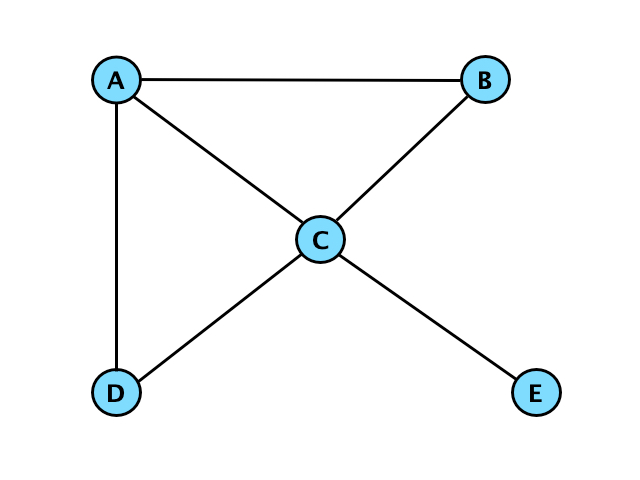
\includegraphics[width=0.8\textwidth]{grafUndir.jpg}
    \caption{Dvosmerne letalske povezave med mesti $A,B,C,D,E$.}
\end{figure}
Če je nadzornik na začetku v mestu $A$, kakšne so verjetnosti, da se v $k$-tem koraku nahaja v mestu $A,B,C,D,E$? Kolikšen delež svojega časa nadzornik preživi v mestih $A,B,C,D,E$ po dolgem času?

Seveda smo že tekom opisa problema zaslutili, da gre za problem iz podpoglavja \ref{podpoglavjeMarkovskeVerige}, ki pa si ga bomo sedaj nekoliko bolj podrobno pogledali. Že v omenjenem podpoglavju smo neusmerjenemu grafu priredili usmerjenega, ki odraža verjetnosti izbire mesta naslednjega postanka.
\begin{figure}[H]
    \centering
    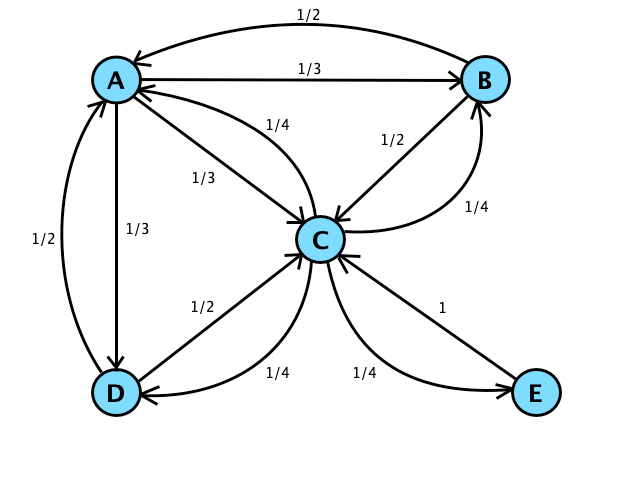
\includegraphics[width=0.8\textwidth]{grafDir.jpg}
    \caption{Usmerjeni graf, ki prikazuje verjetnosti, da bo nadzornik izbral določeno mesto kot naslednji postanek.}
    \label{grafUsmerjeni}
\end{figure}
Problem lahko interpretiramo kot markovsko verigo z množico stanj \[S = \{A, B, C, D, E\}\] in prehodno matriko
\begin{equation*}
    P =
    \kbordermatrix{
            & A & B & C & D & E \\
        A & 0 & 1/3 & 1/3 & 1/3 & 0 \\
        B & 1/2 & 0 & 1/2 & 0 & 0 \\
        C & 1/4 & 1/4 & 0 & 1/4 & 1/4 \\
        D & 1/2 & 0 & 1/2 & 0 & 0 \\
        E & 0 & 0 & 1 & 0 & 0
    },
\end{equation*}
ki je hkrati tudi matrika sosednosti usmerjenega grafa na sliki \ref{grafUsmerjeni}. Z nekoliko truda bi za to matriko izračunali lastne vrednosti
\begin{align*}
    &\lambda_1 = 1, \\
    &\lambda_2 = -\frac{1}{2}, \\
    &\lambda_3 = 0, \\
    &\lambda_4 = \frac{1}{12} \left(-3+\sqrt{33}\right), \\
    &\lambda_5 = \frac{1}{12} \left(-3-\sqrt{33}\right).
\end{align*}
Vse lastne vrednosti razen $\lambda_1$ so po absolutni vrednosti strogo manjši od $1$, torej po izreku \ref{izrekAsimptotika} sledi, da je zaporedje $(P^k)_{k\in\N}$ konvergentno z limito $P_1$, torej spektralnim projektorjem za lastno vrednost $\lambda_1$.

Recimo, da je nadzornik na začetku v mestu $A$. Porazdelitev verjetnosti stanj na $0$-tem koraku bo torej enaka $p(0) = (1, 0, 0, 0, 0)^T$. Po formuli \eqref{eqKtiKorakMarkov} lahko izračunamo porazdelitev verjetnosti stanj na $k$-tem koraku
\begin{equation*}
    p(k) = \left(P^k\right)^T p(0)
\end{equation*}
za vsak $k\in\N$.

Zanima nas še, kakšna je porazdelitev verjetnosti stanj po zelo dolgem času, tj.\ $p(k)$, ko $k\rightarrow\infty$. Vemo, da je
\begin{equation*}
    \lim_{k\rightarrow\infty} P^k = P_1,
\end{equation*}
kjer je $P_1$ spektralni projektor za lastno vrednost $\lambda_1 = 1$. Ker ima matrika $P \in \R^{5 \times 5}$ $5$ različnih lastnih vrednosti, lahko $P_1$ izračunamo po formuli \eqref{spektralniProjektorjiDiag} in dobimo
\begin{equation*}
    P_1 = \frac{1}{2}
    \begin{bmatrix}
        1/2 & 1/3 & 2/3 & 1/3 & 1/6 \\
        1/2 & 1/3 & 2/3 & 1/3 & 1/6 \\
        1/2 & 1/3 & 2/3 & 1/3 & 1/6 \\
        1/2 & 1/3 & 2/3 & 1/3 & 1/6 \\
        1/2 & 1/3 & 2/3 & 1/3 & 1/6
    \end{bmatrix}
    =
    \begin{bmatrix}
        1/4 & 1/6 & 1/3 & 1/6 & 1/12 \\
        1/4 & 1/6 & 1/3 & 1/6 & 1/12 \\
        1/4 & 1/6 & 1/3 & 1/6 & 1/12 \\
        1/4 & 1/6 & 1/3 & 1/6 & 1/12 \\
        1/4 & 1/6 & 1/3 & 1/6 & 1/12
    \end{bmatrix}.
\end{equation*}
Sedaj lahko izračunamo limito $p(k)$, ko gre $k\rightarrow\infty$:
\begin{align*}
    p :&=\lim_{k\rightarrow\infty} p(k) = \lim_{k\rightarrow\infty} \left(P^k\right)^T p(0) = P_1^T\  p(0) = \\
    &= \left(\frac{1}{4}, \frac{1}{6}, \frac{1}{3}, \frac{1}{6}, \frac{1}{12}\right)^T.
\end{align*}
Prva komponenta vektorja $p$ nam pove, kolikšen delež časa bo nadzornik preživel v mestu $A$. Druga komponenta nam pove, kolikšen delež časa bo nadzornik preživel v mestu $B$. Enako sklepamo za mesta $C, D, E$.

\section*{Slovar strokovnih izrazov}

\geslo{A-invarianten podprostor}{A-invariant subspace}
\geslo{Ces\`arova konvergenca}{Ces\`aro summability}
\geslo{koordinatno zaporedje}{coordinate sequence}
\geslo{lastna vrednost}{eigenvalue}
\geslo{lastni vektor}{eigenvector}
\geslo{lastni podprostor}{eigenspace}
\geslo{markovska veriga}{Markov chain}
\geslo{minimalni polinom}{minimal polynomial}
\geslo{množica stanj}{state space}
\geslo{prehodna matrika}{transition matrix}
\geslo{radialno dominantna lastna vrednost}{radially dominant eigenvalue}
\geslo{spekter}{spectrum}
\geslo{spektralna skrčitev}{spectral contraction}
\geslo{spektralni projektor}{spectral projection}
\geslo{spektralni radij}{spectral radius}
\geslo{spektralni razcep}{spectral decomposition}
\geslo{stohastičnost}{stochasticity}

% seznam uporabljene literature
\begin{thebibliography}{99}

\bibitem{kramar} A.~B\'{a}tkai, M.~Kramar Fijavž in A.~Rhandi, \emph{Positive operator semigroups from finite to infinite dimensions}, Birkh\"{a}user/Springer, 2017.

\bibitem{markov} V.~Guruswami in R.~Kannan, \emph{Computer science theory for the information age, Spring 2012}, verzija 2.~2012, [ogled 17.~3.~2021], dostopno na \url{https://www.cs.cmu.edu/~venkatg/teaching/CStheory-infoage/hopcroft-kannan-feb2012.pdf}.

\bibitem{kosir} T.~Košir, \emph{Lastne vrednosti in lastni vektorji (8. poglavje iz predavanj)}, [ogled 17.~3.~2021], dostopno na \url{https://www.fmf.uni-lj.si/~kosir/poucevanje/skripta/lastne.pdf}.

\bibitem{lavric} B.~Lavrič, \emph{Algebra $1$ (kratek pregled rezultatov in definicij)}, [ogled 17.~3.~2021], dostopno na \url{https://www.fmf.uni-lj.si/~lavric/algebra%201%20-%20pregled.pdf}.

\bibitem{bresar} M. Brešar, \emph{Uvod v algebro}, DMFA -- založništvo, Ljubljana, 2018, dostopno tudi na \\ \url{https://www.fmf.uni-lj.si/~bresar/documents/UvodVAlgebro2018.pdf}

\bibitem{meyer} C.~Meyer, \emph{Matrix Analysis and Applied Linear Algebra}, SIAM, 2000.

\bibitem{youtube} HarvardX (28.~2.~2020), Introducing Markov Chains [Video], Youtube, [ogled 10.~10.~2020], dostopno na \url{https://www.youtube.com/watch?v=JHwyHIz6a8A}


\end{thebibliography}

\end{document}

